\part{Complessità}
% LEZIONE 9


\chapter{Introduzione}

Libro di Papadimitriou main reference.

In questa parte utilizzeremo come modello di computazione le \textbf{macchine di Turing} (MdT). Esistono diversi modelli di MdT: macchine di Turing multinastro, macchine di Turing input/output, macchine di Turing con oracolo, macchine di Turing nondeterministiche. Le MdT verranno utilizzate per confrontare i diversi risultati di complessità che possiamo ottenere.

Ci concentreremo sia su \textbf{complessità temporale} (time complexity) che \textbf{spaziale} (space complexity). Il focus non sarà sulla complessità di un dato algoritmo, ma sulla complessità di un problema. I \textbf{problemi} possono essere classificati come di decisione (decision problems), di funzione (function problems), o di ottimizzazione (optimization problems).
\begin{itemize}
    \item \textbf{Decision problem} $P:\text{inputs}\to\{\text{yes},\text{no}\}$
    \item \textbf{Function problem} computare una data funzione, ad esempio l'ordinamento di una lista
    \item \textbf{Optimization problem} tra tutti i possibili output, si vuole trovare quello che minimizza o massimizza una funzione di costo. 
\end{itemize}

\paragraph{Esempio} Sia $G=(V,E)$ un grafo, e $u,v\in V$ due nodi. 
\begin{itemize}
    \item[--] decidere se esiste un cammino da $u$ a $v$ è un problema di decisione
    \item[--] trovare un cammino da $u$ a $v$ è un problema di funzione
    \item[--] trovare il cammino più corto da $u$ a $v$ è un problema di ottimizzazione
\end{itemize}

In questo corso ci concentreremo sui problemi di decisione. Se si ha una soluzione per un problema di funzione o di ottimizzazione, si possiede automaticamente una soluzione per il problema di decisione.\medskip

% (disegno nelle note)
Immaginiamo tutti gli input possibili al problema dell'esempio precedente come ad un insieme infinito di tuple $(G,u,v)$. Questo insieme si può dividere in due: il sottoinsieme dei yes di tutte le codifiche binarie di triple $(G,u,v)$ tali che esiste un cammino in $G$ da $u$ a $v$, e, inversamente, il sottoinsieme no.
\begin{center}
    \begin{tikzpicture}
        \node[ellipse,
            draw,
            minimum width=6cm,
            minimum height=3cm] (A) at (0,0) { };
        \draw (0,-1.5) -- (0,1.5);
        \node[above left] at (A.north west) {$L$};
        \node[below] at (A.220) {yes};
        \node[below] at (A.-40) {no};

        \node at (-2,0.4) {$\bullet$};
        \node at (-0.8,0.2) {$\bullet$};
        \node at (-1.2,-0.4) {$\bullet$};
        \node at (-0.8,-0.8) {$\dots$};
        \node at (1.6,-0.2) {$\bullet$};
        \node at (1.2,0.4) {$\bullet$};
        \node at (0.8,-0.8) {$\dots$};

        \draw[->,decorate,decoration=snake] (-2,0.4) -- (-3.6,1);
        \node[left] at (-3.6,1) {$(G,u,v)$};
    \end{tikzpicture}
\end{center}
La codifica binaria di una tripla è una stringa del tipo $1011\dots$. Più precisamente, è una stringa sull'alfabeto $\Sigma=\{0,1\}$. L'insieme di tutte le possibili stringhe binarie è $\Sigma^*$. Questo insieme è quindi il linguaggio $L$ sottoinsieme di $\Sigma^*$, ovvero $L\subseteq\Sigma^*$.
$$
    L = \{ \bin(G,u,v)|ln~G~u\to v \}
$$

\paragraph{Esempio} Consideriamo interi rappresentati in binario. Vogliamo decidere se un dato intero $x$ è divisibile per 4.
$$
    \bin(x) = 10\dots11
$$
in questo caso non è divisibile per 4. Un numero binario è divisibile per 4 se e solo se i due bit meno significativi sono 0.
$$
    \bin(x) = x_n,x_{n-1},\dots,x_1,x_0 \quad \Leftrightarrow \quad x_0 = 0 \text{ and } x_1 = 0
$$
Il linguaggio indicato da questo problema di decisione è
$$
    L = \{ x\in\{0,1\}^* | x=x_n,x_{n-1},\dots,x_1,x_0 \land x_0 = 0 \land x_1 = 0 \}
$$


\paragraph{Esempio: palindromo} Decidere se una stringa è palindroma, con $\Sigma = \{0,1\}$.
$$
    x_1,x_2,x_3,\dots,x_3,x_2,x_1
$$
Ad esempio, $x=101$ è palindroma, mentre $x=1010$ non lo è. Cerchiamo il linguaggio $L=\{x|x \text{ è palindroma}\}$. Utilizziamo una macchina di Turing.
\begin{center}
    \begin{tikzpicture}
        % Draw the horizontal strip
        \draw (0,0) -- (5,0);
        \draw (0,.5) -- (5,.5);
        %  Draw the squares
        \foreach \x in {0.5,1,...,4.5} {
          \draw (\x,0) -- (\x,.5);
        }

        % Label the squares
        % \foreach \x in {2.25,2.75,3.25,4.25,4.75,5.25} {
        %   \node[above] at (\x,0) {$*$};
        % }
        \node[above] at (0.75,0) {$\rhd$};
        \node[above] at (1.25,0) {$x_1$};
        \node[above] at (1.75,0) {$x_2$};
        \node[above] at (3.75,0) {$x_n$};
        \node[above] at (2.8,0.1) {\Huge \dots};
        \node[above] at (4.25,0) {$\sqcup$};
        \draw [decorate,
            decoration = {brace,mirror,amplitude=5pt}] (1,-0.1) -- (4,-0.1);
        \node[below] at (2.5,-0.2) {$x$};
        \node[below] at (0.75,0) {\LARGE$\substack{\uparrow\\s}$};
        % \node at (0.75,-0.65) {$s$};
    \end{tikzpicture}
\end{center}
Si parte dallo stato $s$ e si vuole finire nello stato $p$ solo quando $x$ è palindroma. Per decidere se $x$ è palindroma, si può leggere $x_1$, ricordarne il valore nello stato del puntatore, e poi confrontarlo con $x_n$. Se sono uguali, si ripete lo stesso procedimento con $x_2$ e $x_{n-1}$, e così via. Se si arriva a $x_n$ e $x_1$ senza aver trovato una discrepanza, allora $x$ è palindroma. Se invece si trova una discrepanza, allora $x$ non è palindroma. Le transizioni sono le seguenti:
\begin{align*}
    \delta(s,\rhd) &= (q,\rhd,\to)\\
    \delta(q,1) &= (q_1,\rhd,\to)\\
    \delta(q,0) &= (q_0,\rhd,\to)\\
\end{align*}
\textcolor{Red}{TODO: finire di scrivere le transizioni}
Questa macchina eseguirà un numero quadratico di passi per controllare se la stringa $x$ è palindroma: $O(|x|^2)$.\medskip

Se si vuole controllare in C (o in un altro linguaggio) se una stringa è palindroma, si può scrivere un programma che confronta il primo e l'ultimo carattere, poi il secondo e il penultimo, e così via, eseguendo un numero lineare di passi. La complessità è $O(|x|)$. Questo è un esempio di come la complessità di un problema dipenda dal modello di computazione utilizzato.


\section{Tesi di Church-Turing Estesa} La tesi di Church-Turing afferma che ogni cosa che può essere computata, può essere computata da una macchina di Turing.

La versione estesa afferma che tutti i modelli (ragionevoli) di calcolo sono correlati polinomialmente. Questo significa che se un problema è risolvibile in tempo polinomiale in un modello di computazione, allora è risolvibile in tempo polinomiale in ogni modello di computazione.

In altre parole, la tesi di Church-Turing estesa afferma che la complessità computazionale di un problema è indipendente dal modello di calcolo utilizzato per risolverlo.
$$
    \underset{\text{problema}}{P} \to \text{MdT }O(f(n)) \to \underset{\text{modello}}{M}~O(p(f(n)))  
$$
Ma è vera anche la direzione contraria. \textcolor{Red}{TODO: ???}




%%%%%%%%%%%%%%%%%%%%%%%%%%%%
\chapter{Macchine di Turing}


\section{Definizioni}

\begin{definition}[Configurazione]
    Una configurazione è una tripla $(q,w,u)$, con
    \begin{itemize}
        \item $q\in K\cup\{\text{yes, no, halt}\}$
        \item $w,u\in\Sigma^*$
    \end{itemize}
\end{definition}
Ad esempio, graficamente, una configurazione è
\begin{center}
    \begin{tikzpicture}
        % Draw the horizontal strip
        \draw (0,0) -- (6,0);
        \draw (0,.5) -- (6,.5);
        %  Draw the squares
        \foreach \x in {0.5,1,1.5,2,3,3.5,4.5,5,5.5} {
          \draw (\x,0) -- (\x,.5);
        }

        \node[above] at (0.75,0) {$\rhd$};
        \node[above] at (1.25,0) {$x_1$};
        \node[above] at (1.75,0) {$x_2$};
        \node[above] at (2.5,0) {\dots};
        \node[above] at (3.25,0) {$x_i$};
        \node[above] at (4,0) {\dots};
        \node[above] at (4.75,0) {$x_n$};
        \node[above] at (5.25,0) {$\sqcup$};
        \draw [decorate,
            decoration = {brace,amplitude=5pt}] (0.5,0.6) -- (3.48,0.6);
        \node[above] at (2,0.7) {$w$};
        \draw [decorate,
            decoration = {brace,amplitude=5pt}] (3.52,0.6) -- (5,0.6);
        \node[above] at (4.25,0.7) {$u$};
        \node[below] at (3.25,0) {\LARGE$\substack{\uparrow\\q}$};
    \end{tikzpicture}
\end{center}


\begin{definition}[Configurazione Iniziale]
    La configurazione iniziale su una stringa $x$ è una tripla 
    $$
    (1,\rhd,x)
    $$
\end{definition}

\begin{definition}[Configurazioni Finali]
    Le configurazioni finali su una stringa $x$ sono una tripla 
    $$
    (H,w,u)
    $$
    dove $H\in\{\text{yes, no, halt}\}$.
\end{definition}


\begin{definition}[Passo di Computazione]
    $$
        (q,w,u) \overset{\delta}{\to} (q',w',u') 
    $$
\end{definition}
Ad esempio, il passo di computazione è $(s,\rhd,001)\to(q,\rhd 0,01)$
\begin{center}
    \begin{tikzpicture}
        % Draw the horizontal strip
        \draw (0,0) -- (4,0);
        \draw (0,.5) -- (4,.5);
        %  Draw the squares
        \foreach \x in {0.5,1,...,3.5} {
          \draw (\x,0) -- (\x,.5);
        };
        \node[above] at (0.75,0) {$\rhd$};
        \node[above] at (1.25,0) {$0$};
        \node[above] at (1.75,0) {$0$};
        \node[above] at (2.25,0) {$1$};
        \node[above] at (2.75,0) {$\sqcup$};
        \node[above] at (3.25,0) {$\sqcup$};
        \node[below] at (0.75,0) {\LARGE\cancel{$\substack{\uparrow\\s}$}};
        \node[below] at (1.25,0) {\LARGE$\substack{\uparrow\\q}$};
    \end{tikzpicture}
\end{center}
Eseguito applicando $\delta(s,\rhd)=(q,\rhd,\to)$.


\begin{definition}[Time Complexity per una MdT $\bm{\mathcal{M}}$ sull'input $\bm{x}$]
    $\mathcal{M}$ ha time complexity $t$ su $x$ se dopo esattamente $t$ passi si raggiunge una configurazione finale.
    $$
        (s,\rhd,x)\underbrace{\to\dots\to}_{t\text{ passi}}(H,w,u)
    $$
    Indicata in breve con $(s,\rhd,x)\to^t(H,w,u)$.\medskip

    \noindent $\mathcal{M}$ ha time complexity $f:\mathbb{N}\to\mathbb{N}$ se, $\forall x\in\Sigma^*$, $(s,\rhd,x)\to^t(H,w,u)$ con $t\leq f(|x|)$.
\end{definition}
La dimensione dell'input (bit length dell'input) è $|x|$. Questa è una complessità nel caso peggiore ($\leq$). Non stiamo utilizzando la notazione big-O.



\section{Unlimited Register Machines}
Una Unlimited Register Machine (URM) è una macchina di Turing con un numero illimitato di registri. 
\begin{table}[H]
    \centering
    \begin{tabular}{c|c|}
    \cline{2-2}
    $R_0$ & $r_0$ \\ \cline{2-2} 
    $R_1$ & $r_1$ \\ \cline{2-2} 
          & \dots \\ \cline{2-2} 
    $R_m$ & $r_m$ \\ \cline{2-2} 
          & \dots 
    \end{tabular}
\end{table}
Ogni registro contiene un numero naturale. Quindi, il contenuto del registro $R_m$ sarà $r_m\in\mathbb{N}$. Le operazioni possibili sono:
\begin{itemize}
    \item \textbf{incremento} $S(i)$: $r_i:=r_i+1$
    \item \textbf{azzeramento} $Z(i)$: $r_i:=0$
    \item \textbf{trasferimento} $T(i,j)$: $r_j:=r_i$, ovvero trasferisco il contenuto del registro $R_i$ nel registro $R_j$
    \item \textbf{jump} $J(i,j,k)$: se $r_i=r_j$ allora salta all'istruzione $k$, altrimenti prosegue con l'istruzione successiva
\end{itemize}

% Macchina con un unbounded number of registers.

% All'inizio, l'input $x$ è in $R_0$. Abbiamo una specie di counter.

\paragraph{Esempio} Dati $x,y\in\mathbb{N}$, decidere se $x=y$.

\subparagraph{MdT} Si può utilizzare una macchina di Turing che contiene la rappresentazione binaria dei due interi, separati da un separatore.
\begin{center}
    \begin{tikzpicture}
        % Draw the horizontal strip
        \draw (0,0) -- (6.5,0);
        \draw (0,.5) -- (6.5,.5);
        %  Draw the squares
        \foreach \x in {0.5,1,1.5,2.5,3,3.5,4,5,5.5,6} {
          \draw (\x,0) -- (\x,.5);
        };
        \node[above] at (0.75,0) {$\rhd$};
        \node[above] at (1.25,0) {$x_1$};
        \node[above] at (2,0) {\dots};
        \node[above] at (2.75,0) {$x_n$};
        \node[above] at (3.25,0) {;};
        \node[above] at (3.75,0) {$y_1$};
        \node[above] at (4.5,0) {\dots};
        \node[above] at (5.25,0) {$y_m$};
        \node[above] at (5.75,0) {$\sqcup$};
        \node[below] at (0.75,0) {\LARGE$\substack{\uparrow\\s}$};
        \draw [decorate,
            decoration = {brace,amplitude=5pt}] (1,0.6) -- (3,0.6);
        \node[above] at (2,0.7) {$x$};
        \draw [decorate,
            decoration = {brace,amplitude=5pt}] (3.5,0.6) -- (5.5,0.6);
        \node[above] at (4.5,0.7) {$y$};
    \end{tikzpicture}
\end{center}
Questa macchina richiede, nel caso peggiore, un numero quadratico di passi per terminare. La com\-ples\-si\-tà è $\Theta(|x|^2)$.

\subparagraph{URM} Possiamo utilizzare una URM con $x$ e $y$ rispettivamente nei registri $R_0$ e $R_1$.
\begin{table}[H]
    \centering
    \begin{tabular}{c|c|}
    \cline{2-2}
    $R_0$ & $x$ \\ \cline{2-2} 
    $R_1$ & $y$ \\ \cline{2-2} 
          &    
    \end{tabular}
\end{table}
\noindent Alla fine, scriveremo 1 in $R_0$ se $x=y$, 0 altrimenti. Le istruzioni sono le seguenti:
\begin{enumerate}
    \item $J(0,1,4)$
    \item $Z(0)$
    \item $J(0,0,100)$
    \item $Z(0)$
    \item $S(0)$
\end{enumerate}
In questo caso, la complessità si può calcolare in due modi.

\begin{definition}[Time Complexity su URM]~
    \begin{itemize}
        \item \emph{Uniform cost criterium} (criterio del costo uniforme): numero di istruzioni eseguite.
        \item \emph{Logarithmic cost criterium} (criterio del costo logaritmico): ogni istruzione ha un costo proporzionale al numero di cifre coinvolte.
    \end{itemize}
\end{definition}
Quindi, per questa macchina, la complessità è 
\begin{itemize}
    \item utilizzando il criterio del costo uniforme: $\Theta(1)$
    \item utilizzando il criterio del costo logaritmico: $\Theta(|x|+|y|)$
\end{itemize}
Nel secondo caso, ci si avvicina al costo per la macchina di Turing. 

Mentre le macchine di Turing sono un modello di computazione sequenziale, nelle URM si ha l'istruzione \emph{jump}. % LEZIONE 10
In altre parole:
\begin{itemize}
    \item \textbf{MdT} 1 bit di informazione in ogni cella $\to$ tempo: numero di passi
    \item \textbf{URM} registri, un intero di lunghezza arbitraria (più bit) in ogni registro $\to$ tempo: numero di istruzioni (uniform time complexity)
\end{itemize}

\paragraph{Esempio} Computare $x+1$, $x\in\mathbb{N}$.
\subparagraph{MdT} Si ha una macchina di Turing che contiene $x$ in binario.
\begin{center}
    \begin{tikzpicture}
        % Draw the horizontal strip
        \draw (0,0) -- (4,0);
        \draw (0,.5) -- (4,.5);
        %  Draw the squares
        \foreach \x in {0.5,1,1.5,2.5,3,3.5} {
          \draw (\x,0) -- (\x,.5);
        };
        \node[above] at (0.75,0) {$\rhd$};
        \node[above] at (1.25,0) {$x_1$};
        \node[above] at (2,0) {\dots};
        \node[above] at (2.75,0) {$x_n$};
        \node[above] at (3.25,0) {$\sqcup$};
        % \node[below] at (0.75,0) {\LARGE$\substack{\uparrow\\s}$};
        \draw [decorate,
            decoration = {brace,amplitude=5pt}] (1,0.6) -- (3,0.6);
        \node[above] at (2,0.7) {$x$};
    \end{tikzpicture}
\end{center}
Nel caso peggiore $x=111\dots1$, quindi la complessità è lineare $\Theta(n)$.

\subparagraph{URM} Si ha una URM con $x$ nel registro $R_0$. È suffieciente una singola istruzione $S(0)$, quindi la complessità è $\Theta(1)$.


\subsection{URM + Prodotto}
Cambiamo il modello di computazione URM, considerando URM + prodotto. Oltre alle istruzioni $S(i)$, $Z(i)$, $T(i,j)$, e $J(i,j,k)$, aggiungiamo l'istruzione $P(i)$, che esegue l'operazione $r_i:=r_i* r_i$.

\paragraph{Esempio di programma per URM + prodotto} Abbiamo in input un numero $x$, che copiamo anche in $R_1$. Applichiamo il prodotto sul contenuto del registro $R_0$ per $x$ volte. In altre parole, vogliamo calcolare $x^{2^x}$.
\begin{enumerate}
    \item $J(1,2,5)$
    \item $P(0)$
    \item $S(2)$
    \item $J(3,3,1)$
\end{enumerate}
Pertendo da un input di $x$ in $R_0$, $x$ in $R_1$, e $0$ in tutti gli altri registri. In un generico passo di iterazione $i$ si avrà:
\begin{table}[H]
    \centering
    \def\arraystretch{1.3}
    \begin{tabular}{c|c|cc|c|cc|c|cc|c|cccc|c|c}
    \cline{2-2} \cline{5-5} \cline{8-8} \cline{11-11} \cline{16-16}
    $R_0$ & $x$      &       & $R_0$ & $x^2$    &       & $R_0$ & $(x^2)^2$ &       & $R_0$ & $(x^4)^2$ &       &         &       & $R_0$ & $x^{2^i}$  \\ \cline{2-2} \cline{5-5} \cline{8-8} \cline{11-11} \cline{16-16} 
    $R_1$ & $x$      &       & $R_1$ & $x$      &       & $R_1$ & $x$       &       & $R_1$ & $x$       &       &         &       & $R_1$ & $x$      \\ \cline{2-2} \cline{5-5} \cline{8-8} \cline{11-11} \cline{16-16} 
    $R_2$ & 0        & ~ $\to$ ~ & $R_2$ & 1        & ~ $\to$ ~ & $R_2$ & 2         & ~ $\to$ ~ & $R_2$ & 3         & ~ $\to$ & $\dots$ & $\to$ ~ & $R_2$ & $i$    \\ \cline{2-2} \cline{5-5} \cline{8-8} \cline{11-11} \cline{16-16} 
    $R_3$ & 0        &       & $R_3$ & 0        &       & $R_3$ & 0         &       & $R_3$ & 0         &       &         &       & $R_3$ & 0        \\ \cline{2-2} \cline{5-5} \cline{8-8} \cline{11-11} \cline{16-16} 
    $R_4$ & $\vdots$ &       & $R_4$ & $\vdots$ &       & $R_4$ & $\vdots$  &       & $R_4$ & $\vdots$  &       &         &       & $R_4$ & $\vdots$
    \end{tabular}
\end{table}
Il numero di istruzioni è lineare $\Theta(n)$.

\subparagraph{MdT} Se si eseguisse la stessa computazione su una macchina di Turing, si avrebbe 
\begin{center}
    \begin{tikzpicture}
        % Draw the horizontal strip
        \draw (0,2) -- (4,2);
        \draw (0,2.5) -- (4,2.5);
        %  Draw the squares
        \foreach \x in {0.5,1,1.5,2.5,3,3.5} {
          \draw (\x,2) -- (\x,2.5);
        };
        \node[above] at (0.75,2) {$\rhd$};
        \node[above] at (1.25,2) {$x_1$};
        \node[above] at (2,2) {\dots};
        \node[above] at (2.75,2) {$x_n$};
        \node[above] at (3.25,2) {$\sqcup$};
        \draw [decorate,
            decoration = {brace,amplitude=5pt}] (1,2.6) -- (3,2.6);
        \node[above] at (2,2.7) {$x$};

        \node at (2,1.3) {$\vdots$};

        % Draw the horizontal strip
        \draw (0,0) -- (4,0);
        \draw (0,.5) -- (4,.5);
        %  Draw the squares
        \foreach \x in {0.5,1,1.5,2.5,3,3.5} {
          \draw (\x,0) -- (\x,.5);
        };
        \node[above] at (0.75,0) {$\rhd$};
        \node[above] at (1.25,0) {$y_1$};
        \node[above] at (2,0) {\dots};
        \node[above] at (2.75,0) {$y_m$};
        \node[above] at (3.25,0) {$\sqcup$};
        \draw [decorate,
            decoration = {brace,mirror,amplitude=5pt}] (1,-.1) -- (3,-.1);
        \node[below] at (2,-.2) {$x^{2^x}$};
    \end{tikzpicture}
\end{center}
Quindi $\Omega(\log(x^{2^x}))=\Omega(2^x \log(x))$.\bigskip

Questo risultato sembra contraddire la tesi di Church-Turing estesa, che afferma che tutti i modelli \textbf{ragionevoli} di computazione sono correlati polinomialmente. Ma cosa significa \emph{ragionevole}? Non si può avere una operazione che fa crescere ``troppo'' l'input (nell'esempio, il prodotto), si deve utilizzare il criterio logaritmico.

In altre parole, se l'algoritmo utilizza operazioni che in un numero polinomiale di passi fanno crescere l'input esponenzialmente, e queste sono utilizzate un numero di volte che dipende dalla dimensione dell'input, allora si deve utilizzare un criterio logaritmico. Quando non si è sicuri della potenza delle operazioni della macchina, il costo di ogni singola operazione dev'essere proporzionale al numero di bit manipolati.
\begin{table}[H]
    \centering
    \def\arraystretch{1.3}
    \begin{tabular}{ccc}
    \rowcolor[HTML]{C0C0C0} 
    istruzione & uniform     & logarithmic                        \\
    $S(i)$     & $\Theta(1)$ & $\Theta(\log(r_i))$                \\
    \rowcolor[HTML]{EFEFEF} 
    $Z(i)$     & $\Theta(1)$ & $\Theta(1)$                        \\
    $T(i,j)$   & $\Theta(1)$ & $\Theta(\log(r_i))$                \\
    \rowcolor[HTML]{EFEFEF} 
    $J(i,j,k)$ & $\Theta(1)$ & $\Theta(\min(\log(r_i),\log(r_j)))$\\
    $P(i)$     & $\Theta(1)$ & $\Theta((\log(r_i))^2)$            
    \end{tabular}
\end{table}
Con $r_i$ contenuto del registro $i$. In particolare per $P(i)$, nella moltiplicazione di un numero $x$ per se stesso si ha $x_1,x_2,\dots,x_n \times x_1,x_2,\dots,x_n$. Si hanno $x^n$ bit operazioni, quindi $O((\log(x))^2)$.



\section{Ulteriori Definizioni}
Come abbiamo visto, nei problemi di decisione si ha un input $x\in\Sigma^*$ e un output in $\{\text{yes},\text{no}\}$. Possiamo definire un linguaggio $L$ come l'insieme di tutte le stringhe che hanno output yes. 
$$
    L \subseteq (\Sigma \backslash \{ \sqcup \} )^*
$$
Un problema $P$ è una funzione
$$
    P:\Sigma^*\to\{\text{yes},\text{no}\}
$$

\begin{definition}[Linguaggio Ricorsivo]
    \begin{eqnarray*}
        &\text{Una macchina di Turing $\mathcal{M}$ decide un linguaggio $L$}&\\
        &\Updownarrow&\\
        &\forall x\in(\Sigma\backslash\{\sqcup\})^* \begin{cases*}
            x\in L \to \mathcal{M}(x)=\text{yes}\\
            x\notin L \to \mathcal{M}(x)=\text{no}
        \end{cases*}&
    \end{eqnarray*}
    Il linguaggio $L$ si dice \textbf{ricorsivo}.
\end{definition}

\begin{definition}[Linguaggio Ricorsivamente Enumerabile]
    \begin{eqnarray*}
        &\text{Una macchina di Turing $\mathcal{M}$ accetta un linguaggio $L$}&\\
        &\Updownarrow&\\
        &\forall x\in(\Sigma\backslash\{\sqcup\})^* \begin{cases*}
            x\in L \to \mathcal{M}(x)=\text{yes}\\
            x\notin L \to \mathcal{M}(x)\uparrow \text{ (non termina)}
        \end{cases*}&
    \end{eqnarray*}
    Il linguaggio $L$ si dice \textbf{ricorsivamente enumerabile}.
\end{definition}

\begin{theorem}
    $$
        \text{$L$ è ricorsivo } \Rightarrow \text{ $L$ è ricorsivamente enumerabile}
    $$
\end{theorem}

\paragraph{Esempio} Trovare un linguaggio $L$ tale che $L$ è ricorsivamente enumerabile ma non ricorsivo.

Nell'halting problem abbiamo 
$$
    \mathcal{U}(\mathcal{M};x)=\mathcal{M}(x)
$$
L'halting language
$$
    H = \{ (\bin(\mathcal{M});x) ~|~ \mathcal{M}(x)\downarrow \}
$$
è ricorsivamente enumerabile ma non ricorsivo. Infatti, se $\mathcal{M}$ termina su $x$, allora $\mathcal{U}(\mathcal{M};x)=\mathcal{M}(x)=\text{yes}$, altrimenti $\mathcal{U}(\mathcal{M};x)\uparrow$. Questo è un risultato qualitativo.

\paragraph{Esempio} Sia
$$
    L = \{ \bin(\mathcal{M}) ~|~ \forall x~\mathcal{M}(x)\downarrow \text{ in al massimo 100 passi} \}
$$
$L$ è ricorsivo. Infatti, la macchina $\mathcal{M}$ può eseguire al massimo 100 spostamenti a destra sul nastro. Quindi, tutte le macchine che terminano in al massimo 100 passi accettano input $\forall x\in|\Sigma|^n$ con $n\leq 100$.

\begin{definition}[Computazione di Funzioni]
    Sia $f$ una funzione $f:(\Sigma\backslash\sqcup)^*\to\Sigma^*$. Una macchina di Turing $\mathcal{M}$ computa $f$ se
    $$
        \forall x\in(\Sigma\backslash\sqcup)^*\qquad \mathcal{M}(x)\downarrow \text{ e alla fine $f(x)$ è sul nastro}
    $$
    La funzione $f$ è detta \textbf{ricorsiva}, o \textbf{computabile}.
\end{definition}


\section{Macchine di Turing a $k$-nastri e Input/Output}
\begin{definition}[Macchina di Turing a $k$-nastri]
    Una macchina di Turing a $k$-nastri è u\-na tupla $\mathcal{M}=(K,\Sigma,\delta,s)$ con $K,\Sigma,s$ definite come per una macchina di Turing, e
    $$
        \delta : K\times\Sigma \to (K\cup\{\text{yes},\text{no},\text{halt}\}) \times
                                    (\Sigma \times \{\gets,\to,-\})^k
    $$    
\end{definition}
Una macchina di Turing a $k$-nastri è una macchina di Turing con un numero limitato di nastri, che possono essere utilizzati in parallelo. La funzione $\delta$ cambia perché si ha un puntatore per nastro.
\begin{center}
    \begin{tikzpicture}
        \draw (0,2) -- (4,2);
        \draw (0,2.5) -- (4,2.5);
        \foreach \x in {0.5,1,1.5,2} {
          \draw (\x,2) -- (\x,2.5);
        };
        \node[above] at (0.75,2) {$\rhd$};
        \node[above] at (2.5,2) {\dots};
        \node[below] at (1.25,2) {$\uparrow$};

        \draw (0,.75) -- (4,.75);
        \draw (0,1.25) -- (4,1.25);
        \foreach \x in {0.5,1,1.5,2} {
          \draw (\x,.75) -- (\x,1.25);
        };
        \node[above] at (0.75,.75) {$\rhd$};
        \node[above] at (2.5,.75) {\dots};
        \node[below] at (3.25,.75) {$\uparrow$};

        \node at (2,.2) {$\vdots$};

        \draw (0,-.5) -- (4,-.5);
        \draw (0,-1) -- (4,-1);
        \foreach \x in {0.5,1,1.5,2} {
          \draw (\x,-.5) -- (\x,-1);
        };
        \node[above] at (0.75,-1) {$\rhd$};
        \node[above] at (2.5,-1) {\dots};
        \node[below] at (0.75,-1) {$\uparrow$};

        \draw [decorate,
            decoration = {brace,amplitude=5pt}] (-.3,-1.5) -- (-.3,2.5);
        \node at (-.7,.5) {$k$};
    \end{tikzpicture}
\end{center}

\begin{definition}[Macchina di Turing a $k$-nastri con Input/Output]
    Una macchina di\\Turing a $k$-nastri con I/O è una macchina di Turing a $k$-nastri con un nastro di input e un nastro di output. Il nastro di input è di sola lettura, il nastro di output è di sola scrittura.
\end{definition}
\begin{center}
    \begin{tikzpicture}
        \draw (0,2) -- (4,2);
        \draw (0,2.5) -- (4,2.5);
        \foreach \x in {0.5,1,1.5,2} {
          \draw (\x,2) -- (\x,2.5);
        };
        \node[above] at (0.75,2) {$\rhd$};
        \node[above] at (2.5,2) {\dots};
        \node[below] at (1.25,2) {$\uparrow$};

        \draw (0,.75) -- (4,.75);
        \draw (0,1.25) -- (4,1.25);
        \foreach \x in {0.5,1,1.5,2} {
          \draw (\x,.75) -- (\x,1.25);
        };
        \node[above] at (0.75,.75) {$\rhd$};
        \node[above] at (2.5,.75) {\dots};
        \node[below] at (3.25,.75) {$\uparrow$};

        \node at (2,.2) {$\vdots$};

        \draw (0,-.5) -- (4,-.5);
        \draw (0,-1) -- (4,-1);
        \foreach \x in {0.5,1,1.5,2} {
          \draw (\x,-.5) -- (\x,-1);
        };
        \node[above] at (0.75,-1) {$\rhd$};
        \node[above] at (2.5,-1) {\dots};
        \node[below] at (0.75,-1) {$\uparrow$};

        \draw [decorate,
            decoration = {brace,amplitude=5pt}] (-.3,-1.5) -- (-.3,2.5);
        \node at (-.7,.5) {$k$};

        \node[right] at (4.25,2.25) {input};
        \node[right] at (4.25,-.75) {output};
    \end{tikzpicture}
\end{center}

\begin{definition}[Configurazione e Configurazione Iniziale]
    Siano $w_i,u_i\in\Sigma^*$ stringhe. Una configurazione è una tupla
    $$
        (q,w_1,u_1,w_2,u_2,\dots,w_k,u_k)
        \to 
        (q',w_1',u_1',w_2',u_2',\dots,w_k',u_k')
    $$
    Una configurazione iniziale su input $x$ è una tupla
    $$
        (s,\rhd,x,\rhd,\varepsilon,\dots,\rhd,\varepsilon)
    $$
\end{definition}



% LEZIONE 11
\subsection{Complessità Temporale}
Ricordiamo che $L$ è deciso dalla macchina a $k$-nastri $\mathcal{M}$ se, $\forall x$,
\begin{eqnarray*}
    x\in L &\to& \mathcal{M}(x)=\text{yes}\\
    x\notin L &\to& \mathcal{M}(x)=\text{no}
\end{eqnarray*}
Inoltre,
$$
    \underbrace{(s,\rhd,x,\rhd,x,\dots)}_{\text{conf.~iniziale}}
     ~\to^{\mathcal{M}_t}
    \underbrace{(H,\dots)}_{\text{conf.~finale}}
    \qquad
    H\in\{\text{yes},\text{no}\}, \quad 
    \forall x ~~ t\leq f(|x|)
$$
$\mathcal{M}$ indica $L$ in tempo al massimo $f(n)$.

\paragraph{Esempio: palindromo} Consideriamo $\mathcal{M}_1$ macchina di Turing a singolo nastro vs $\mathcal{M}_2$ macchina di Turing a $k$-nastri. Sia $L$ il linguaggio di palindromi su $\{0,1\}$. Le complessità temporali sono 
\begin{itemize}
    \item $\mathcal{M}_1$: $\Theta(n^2)$
    \item $\mathcal{M}_2$: $\Theta(n)$
\end{itemize}
Vedremo come il risultato generale indica che questo è il peggior incremento che si può ottenere.

\begin{theorem}
    \begin{eqnarray*}
        &L \text{ è deciso da una macchina di Turing a } k \text{-nastri } \mathcal{M} \text{ in tempo } f(n)&\\
        &\Downarrow&\\
        &\exists \text{ una macchina di Turing a 1-nastro } \mathcal{M}' \text{ che decide } L \text{ in tempo (al massimo) } O(f(n)^2)&
    \end{eqnarray*}
\end{theorem}

\paragraph{Dimostrazione} Sia $\mathcal{M}$ macchina di Turing a $k$-nastri che decide $L$ in tempo $f(n)$. Vogliamo costruire una macchina di Turing a 1-nastro $\mathcal{M}'$ in grado di simularla. Si possono rappresentare le informazioni dei $k$-nastri su un singolo nastro in questo modo:
\begin{center}
    \begin{tikzpicture}
        \draw (0,-1) -- (8,-1);
        \draw (0,-.5) -- (8,-.5);
        \foreach \x in {0.5,1} {
          \draw (\x,-1) -- (\x,-.5);
        };
        \node[above] at (0.75,-1) {$\rhd$};
        \node[above] at (5,-1) {$\dots$};
        \node[ellipse,
            draw,
            minimum width=1.6cm,
            minimum height=.75cm] (A) at (1.75,-.75) { };
        \node[ellipse,
            draw,
            minimum width=1.6cm,
            minimum height=.75cm] (A) at (3.4,-.75) { };
        \node[ellipse,
            draw,
            minimum width=1.6cm,
            minimum height=.75cm] (A) at (6.5,-.75) { };
        \node[below] at (1.75,-1.1) {nastro 1};
        \node[below] at (3.4,-1.1) {nastro 2};
        \node[below] at (6.5,-1.1) {nastro $k$};
        \node[left] at (-.3,-.75) {$\mathcal{M}'$};
    \end{tikzpicture}
\end{center}
Per imitare i vari cursori, si può ingrandire l'alfabeto:
$$
    \Sigma \cup \underline{\Sigma} \cup \{\rhd'\}
    \qquad 
    \underline{\Sigma} = \{ \underline{\sigma}|\sigma\in\Sigma \}
$$
In ogni momento la macchina $\mathcal{M}$ legge $k$ simboli in $\mathcal{M}'$, bisogna leggere tutto il nastro per leggere (e memorizzare) il valore di tutti i $k$ simboli, e poi un ulteriore scansione per cambiarli. In altre parole, per simulare un passo di $\mathcal{M}$ su $\mathcal{M}'$:
\begin{itemize}
    \item Scansionare il nastro di $\mathcal{M}'$ per leggere i $\underline{\sigma}$ e memorizzarli nello stato di $\mathcal{M}'$
    \item Tornare indietro
    \item Cambiare i $\underline{\sigma}$
    \begin{itemize}
        \item Ad esempio, se nel nastro in $\mathcal{M}$ cambio un simbolo e mi muovo a destra ($\to$), in $\mathcal{M}'$ passerò da 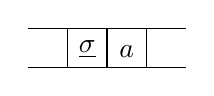
\begin{tikzpicture}\draw (0,0) -- (2,0);
            \draw (0,.5) -- (2,.5);
            \foreach \x in {0.5,1,1.5} {
              \draw (\x,0) -- (\x,.5);
            };
            \node[above] at (0.75,0) {$\underline{\sigma}$};
            \node[above] at (1.25,0) {$a$};\end{tikzpicture}
        a 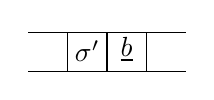
\begin{tikzpicture}\draw (0,0) -- (2,0);
            \draw (0,.5) -- (2,.5);
            \foreach \x in {0.5,1,1.5} {
              \draw (\x,0) -- (\x,.5);
            };
            \node[above] at (0.75,0) {$\sigma'$};
            \node[above] at (1.25,0) {$\underline{b}$};\end{tikzpicture}
    \end{itemize}
\end{itemize} 
Nel caso peggiore, ognuno dei $k$ cambiamenti richiede di spostare tutto a destra per creare spazio sul nastro di $\mathcal{M}'$. 

La domanda ora è: quanto è lungo al massimo il nastro di $\mathcal{M}'$ durante la computazione? Per $k-1$ nastri si ha un'occupazione che è al massimo $f(n)$, e per il primo nastro $n+f(n)$, con $n$ lunghezza dell'input. Quindi, con l'ipotesi che $f(n)\geq n$, si ha 
$$
(k-1)\cdot O(f(n)) + O(n+f(n)) = kO(f(n)) = O(f(n))
$$
Si può concludere che simulare un passo di $\mathcal{M}$ richiede tempo $O(f(n))$. Poiché ci vogliono $O(f(n))$ passi di $\mathcal{M}'$ per simulare un passo di $\mathcal{M}$, si ha che $\mathcal{M}'$ decide $L$ in tempo $O(f(n)^2)$. \hfill $\square$\medskip

A seguito di questo risultato, d'ora in poi si farà affidamento solo sulla complessità delle macchine di Turing a $k$-nastri.

\begin{definition}[Appartenenza ad una Classe di Complessità Temporale]
    $$
        L\in\text{TIME}(f(n)) ~ \exists \text{ MdT a } k \text{-nastri } \mathcal{M} \text{ che decide } L \text{ in tempo } f(n)
    $$
\end{definition}
Ad esempio, Palindromi $\in$ TIME$(3n+4)$. Questo insieme di linguaggi potrebbe essere diverso da, ad esempio, TIME$(2n+1)$. Non utilizziamo la notazione asintotica.

\begin{theorem}[Speed-Up Theorem per TIME]
    $$
        L\in\text{TIME}(f(n))
        ~\Rightarrow~
        \forall\varepsilon>0\quad L\in\text{TIME}(f'(n))
    $$
    con $f'(n)=\varepsilon\cdot f(n)+n+2$.
\end{theorem}
Bisogna sempre pagare il tempo lineare $n+2$ per leggere l'input. Questo risultato ci dice che possiamo utilizzare la notazione asintotica.

\paragraph{Dimostrazione} Sia $\mathcal{M}$ macchina di Turing a $k$-nastri che decide $L$ in tempo $f(n)$. Vogliamo costruire una macchina di Turing a $k$-nastri $\mathcal{M}'$ che simula $m$ passi di $\mathcal{M}$ in ``un singolo passo'' (nel libro sono fissati 6 passi). Ad esempio, se $f(n)=3n^2$ e $\varepsilon=\frac{1}{3}$, allora $f'(n)=n^2$.

Vogliamo codificare blocchi di $m$ passi in un singolo passo: $\Sigma'=\Sigma^m$. Quando $\mathcal{M}'$ legge una cella, sta in realtà leggendo $m$ simboli. 
\begin{itemize}
    \item Si copia il nastro di input da $\mathcal{M}$ a $\mathcal{M}'$, e lo si traduce da $\Sigma$ a $\Sigma'$: questo costa $n+1$.
    \item Per quanto riguarda il puntatore, sappiamo che in $\mathcal{M}$ gli stati sono in $K$, mentre in $\mathcal{M}'$ sono in $K\times\{1,\dots,m\}^k$. In $\mathcal{M}'$ devo sapere dove sta il puntatore, ma se in $\mathcal{M}$ viene letto qualcosa nei successivi $m$ passi (si cambia quindi di cella in $\mathcal{M}'$), gli stati di $\mathcal{M}'$ sono in $K\times\{1,\dots,m\}^k\times (\Sigma^m)^2k$.
\end{itemize}
I passi di $\mathcal{M}'$ sono quindi $n+2+f(n)\cdot\varepsilon$. \hfill $\square$\medskip

Abbiamo cambiato architettura, ciò che si può memorizzare in una singola cella. Ad esempio, se costruiamo una macchina in cui $m=18$, 18 passi di $\mathcal{M}$ vengono simulati da 6 passi di $\mathcal{M}'$. Quindi i passi di $\mathcal{M}'$ sono $n+2+f(n)\cdot\frac{6}{m}$, con $\frac{6}{m}=\varepsilon$.



% \textcolor{Red}{TODO: finire lezione 11}


% LEZIONE 12
\subsection{Complessità Spaziale}
Una configurazione finale di una macchina di Turing a $k$-nastri è del tipo $(H,w_1,u_1,\dots,w_k,u_k)$. Include anche tutte le parti raggiunte durante la computazione (anche se tutti i cursori alla fine puntano a $\sqcup$). Si può utilizzare come complessità spaziale la lunghezza della configurazione finale.

\begin{definition}[Complessità Spaziale per una MdT a $k$-nastri su input $x$]
    Si ha che
    $$
        (s,\rhd,x) \to^* (H,w_1,u_1,\dots,w_k,u_k)
    $$
    con $H=\{\text{halt},\text{yes},\text{no}\}$. Lo spazio utilizzato è
    $$
        \sum_{i=1}^k |w_i| + |u_i|
    $$
\end{definition}
Se non vogliamo contare la dimensione dell'input e dell'output, bisogna utilizzare le macchine di Turing a $k$-nastri con I/O. L'input può essere solo letto, e l'output solo scritto.

\begin{definition}[Complessità Spaziale per una MdT a $k$-nastri con I/O]
    Si ha che
    $$
        (s,\rhd,x) \to^* (H,w_1,u_1,\dots,w_k,u_k)
    $$
    con $H=\{\text{halt},\text{yes},\text{no}\}$. Lo spazio utilizzato è
    $$
        \sum_{i=2}^{k-1} |w_i| + |u_i|
    $$
\end{definition}
dove $\delta(q,\sigma_1,\dots,\sigma_k)=(q',\sigma_1',\dots,\sigma_k',\to)$.

\begin{definition}[Classi di Complessità Spaziale]
    $L$ è decidibile in spazio $f(n)$ se esiste una macchina di Turing a $k$-nastri con I/O $\mathcal{M}$ che decide $L$ e, $\forall x$, $\mathcal{M}$ utilizza uno spazio al massimo $f(|x|)$.
\end{definition}

\paragraph{Esempio: palindromo} $L=\{x|x\text{ è palindroma}\}$. Si vuole trovare la macchina più efficiente in termini di spazio. La seguente macchina è efficiente nel tempo:
\begin{center}
    \begin{tikzpicture}
        \draw (0,1) -- (4.5,1);
        \draw (0,1.5) -- (4.5,1.5);
        \foreach \x in {0.5,1,1.5,3,3.5,4} {
          \draw (\x,1) -- (\x,1.5);
        };
        \node[above] at (0.75,1) {$\rhd$};
        \node[above] at (1.25,1) {$x_1$};
        \node[above] at (2.25,1) {\dots};
        \node[above] at (3.25,1) {$x_n$};
        \node[above] at (3.75,1) {$\sqcup$};

        \draw (0,0) -- (4.5,0);
        \draw (0,.5) -- (4.5,.5);
        \foreach \x in {0.5,1,1.5,3,3.5,4} {
          \draw (\x,0) -- (\x,.5);
        };
        \node[above] at (0.75,0) {$\rhd$};
        \node[above] at (1.25,0) {$x_1$};
        \node[above] at (2.25,0) {\dots};
        \node[above] at (3.25,0) {$x_n$};
        \node[above] at (3.75,0) {$\sqcup$};

        \draw[->] (4.6,1.25) to[out=0,in=0,distance=20] (4.6,.25);
        \node[right] at (5.1,.75) {copia};

        \node[left] at (-.25,1.25) {input};
        \node[left] at (-.25,.25) {working tape};
    \end{tikzpicture}
\end{center}
perché ha $\text{TIME }\Theta(n)$ e $\text{SPACE }\Theta(n)$. Mentre la seguente macchina è efficiente nello spazio:
\begin{center}
    \begin{tikzpicture}
        \draw (0,1) -- (5.5,1);
        \draw (0,1.5) -- (5.5,1.5);
        \foreach \x in {0.5,1,1.5,4,4.5,5} {
          \draw (\x,1) -- (\x,1.5);
        };
        \node[above] at (0.75,1) {$\rhd$};
        \node[above] at (1.25,1) {$\cancel{x_1}$};
        \node[above] at (1.25,1.5) {$\rhd$};
        \node[above] at (2.75,1) {\dots};
        \node[above] at (4.25,1) {$\cancel{x_n}$};
        \node[above] at (4.25,1.5) {$\sqcup$};
        \node[above] at (4.75,1) {$\sqcup$};

        \draw (0,0) -- (5.5,0);
        \draw (0,.5) -- (5.5,.5);
        \foreach \x in {0.5,1,1.5,2.5,3,4,4.5,5} {
          \draw (\x,0) -- (\x,.5);
        };
        \node[above] at (0.75,0) {$\rhd$};
        \node[above] at (1.25,0) {$x_1$};
        \node[above] at (2,0) {\dots};
        \node[above] at (2.75,0) {$x$};
        \node[above] at (3.5,0) {\dots};
        \node[above] at (4.25,0) {$x_n$};
        \node[above] at (4.75,0) {$\sqcup$};

        \draw (0,-1) -- (5.5,-1);
        \draw (0,-.5) -- (5.5,-.5);
        \foreach \x in {0.5,1,1.5,2.5,3,4,4.5,5} {
          \draw (\x,-1) -- (\x,-.5);
        };
        \node[above] at (0.75,-1) {$\rhd$};
        \node[above] at (1.25,-1) {$x_1$};
        \node[above] at (2,-1) {\dots};
        \node[above] at (2.75,-1) {$x$};
        \node[above] at (3.5,-1) {\dots};
        \node[above] at (4.25,-1) {$x_n$};
        \node[above] at (4.75,-1) {$\sqcup$};

        \draw [decorate,
            decoration = {brace,mirror,amplitude=5pt}] (.5,-1.1) -- (3,-1.1);
        \node[below] at (1.75,-1.25) {$y$};
    \end{tikzpicture}
\end{center}
con $\text{SPACE }\Theta(\log n)$.\bigskip

\begin{definition}
    \begin{align*}
        \text{TIME}(f(n)) = \{ L~|~L\text{ può essere deciso in tempo }f(n) \}\\
        \text{SPACE}(f(n)) = \{ L~|~L\text{ può essere deciso in spazio }f(n) \}
    \end{align*}
\end{definition}
In altre parole, $\text{SPACE}(f(n))$ è l'insieme di tutti i linguaggi che possono essere decisi in tempo $f(n)$ da una macchina di Turing a $k$-nastri con I/O. Per ogni input $x$ tale che $|x|=n$, la macchina utilizza spazio al più $f(n)$. 
\begin{property}
    Se esiste una macchina di Turing che decide $L$ in tempo $f(n)$, e $f(n)\geq n$, al\-lo\-ra esiste una macchina di Turing con I/O che decide $L$ in tempo $O(f(n))$.
\end{property}

\paragraph{Esempio} Calcola $x+y$.
\begin{center}
    \begin{tikzpicture}
        \draw (0,1) -- (7,1);
        \draw (0,1.5) -- (7,1.5);
        \foreach \x in {0.5,1,1.5,2,3,3.5,4,4.5,5.5,6,6.5} {
          \draw (\x,1) -- (\x,1.5);
        };
        \node[above] at (0.75,1) {$\rhd$};
        \node[above] at (1.25,1) {$x_1$};
        \node[above] at (1.75,1) {$x_2$};
        \node[above] at (2.5,1) {\dots};
        \node[above] at (3.25,1) {$x_r$};
        \node[above] at (3.75,1) {;};
        \node[above] at (4.25,1) {$y_1$};
        \node[above] at (5,1) {\dots};
        \node[above] at (5.75,1) {$y_m$};
        \node[above] at (6.25,1) {$\sqcup$};

        \draw [decorate,
            decoration = {brace,amplitude=5pt}] (1,1.6) -- (6,1.6);
        \node[above] at (3.5,1.75) {$n$};

        \node at (3.5,0.3) {\vdots};

        \draw (0,-1) -- (7,-1);
        \draw (0,-.5) -- (7,-.5);
        \foreach \x in {0.5,1,1.5,5.5,6,6.5} {
          \draw (\x,-1) -- (\x,-.5);
        };
        \node[above] at (0.75,-1) {$\rhd$};
        \node[above] at (1.25,-1) {$z_1$};
        \node[above] at (3.5,-1) {\dots};
        \node[above] at (5.75,-1) {$z_n$};
        \node[above] at (6.25,-1) {$\sqcup$};

        \draw [decorate,
            decoration = {brace,amplitude=5pt}] (-.2,-.3) -- (-.2,.8);
        \node[left] at (-.35,.25) {working tapes};

        \node[right] at (7.2,1.25) {input};
        \node[right] at (7.2,-.75) {output};
    \end{tikzpicture}
\end{center}
Questo ha spazio lineare $\Theta(n)$ (molto male).\bigskip

\begin{definition}[Classe P]
    Definiamo la classe P come
    $$
        \text{P} = \bigcup_{h\in\mathbb{N}} \text{TIME}(n^h)
    $$
    ovvero l'unione di tutti i problemi che possono essere risolti in tempo polinomiale.
\end{definition}
La classe P ci piace così tanto perché abbiamo la tesi di Church-Turing estesa. Questa classe è \textbf{invariante} rispetto alla scelta del modello di computazione.
Possiamo definire la classe EXP
$$
    \text{EXP} = \bigcup_{h\in\mathbb{N}} \text{TIME}(2^{n^h})
$$

La classe $\mathbb{L}$, PSPACE, e EXPSPACE
\begin{align*}
    \mathbb{L} &= \text{SPACE}(\log n)\\
    \text{PSPACE} &= \bigcup_{h\in\mathbb{N}} \text{SPACE}(n^h)\\
    \text{EXPSPACE} &= \bigcup_{h\in\mathbb{N}} \text{SPACE}(2^{n^h}) 
\end{align*}

\begin{property}~
    $$
        \text{TIME}(f(n)) \subseteq \text{SPACE}(f(n))
    $$    
\end{property}

% book, section 2.6
\section{Random Access Machines}
Capitolo 2.6 del libro. Le random access machine (RAM), sono un modello di computazione sequenziale, composte da registri di input e registri di lavoro. Ogni registro contiene un intero.
\begin{table}[H]
    \centering
    \def\arraystretch{1.5}
    \begin{tabular}{lc|c|clc|c|}
        \cline{3-3} \cline{7-7}
        registri di input & $I_1$    & $\qquad$ & $\qquad$ & working registers & $R_0$    & $\qquad$ \\ \cline{3-3} \cline{7-7} 
                          & $\vdots$ &          &          &                   & $\vdots$ &          \\ \cline{3-3} \cline{7-7} 
                          & $R_i$    &          &          &                   & $I_j$    &          \\ \cline{3-3} \cline{7-7} 
                          & $\vdots$ &          &          &                   & $\vdots$ &         
    \end{tabular}
\end{table}

\noindent Le operazioni possibili sono:
\begin{itemize}
    \item \texttt{READ} $j$: $r_0:=i_j$
    \item \texttt{READ} $\uparrow j$: $r_0:=i_{r_j}$ (vai al registro $R_j$, leggine il contenuto $h$, vai al registro $I_h$, copiane il contenuto in $R_0$)
    \item \texttt{STORE} $j$: $r_j:=r_0$
    \item \texttt{STORE} $\uparrow j$
    \item \texttt{LOAD} $j$: $r_0:=r_j$
    \item \texttt{LOAD} $\uparrow j$
    \item \texttt{LOAD} $=j$: $r_0:=j$
    \item \texttt{ADD} $j$: $r_0:=r_0+r_j$
    \item \texttt{ADD} $\uparrow j$: $r_0:=r_0+r_{r_j}$ 
    \item \texttt{ADD} $=j$
    \item \texttt{SUB} $j$
    \item \dots
    \item \texttt{HALF}: $r_0:=\left\lfloor \dfrac{r_0}{2} \right\rfloor$ (tolgo da $r_0$ l'ultimo bit)
    \item \texttt{JUMP} $j$: $k:=j$ (contatore)
    \item \texttt{JPOS} $j$: if $r_0>0$ then $k:=j$
    \item \texttt{JNEG} $j$
    \item \texttt{JZERO} $j$
    \item \texttt{HALT}
\end{itemize}
Il libro dimostra che
\begin{theorem}
    RAM con complessità temporale uniforme e macchine di Turing con $k$-nastri sono correlate polinomialmente.
\end{theorem}
In particolare 
\begin{align*}
    \underbrace{\text{MdT}}_{f(n)} &\to^{\text{simula}} \underbrace{\text{RAM}}_{O(f(n))}\\
    \underbrace{\text{RAM}}_{f(n)} &\to^{\text{simula}} \underbrace{\text{MdT a 7-nastri}}_{O((f(n))^3)}\\
\end{align*}
Ad esempio, quando si sommano due numeri, si ottiene al massimo 1 bit in più dell'input maggiore.

% LEZIONE 13
\section{Macchine Nondeterministiche}
Si hanno
\begin{itemize}
    \item Macchine deterministiche $\mathcal{M}=(K,\Sigma,\delta,s)$, con $\delta$ \textbf{funzione}
    $$
        \delta:K\times\Sigma^k\to (K\cup\{\text{yes},\text{no},\text{halt}\}) \times \Sigma^k \times \{\gets,\to,-\}^k
    $$
    la cui configurazione è del tipo
    $$
        c \to c'
    $$
    \item Macchine nondeterministiche $\mathcal{N}=(K,\Sigma,\Delta,s)$, con $\Delta$ \textbf{relazione}
    $$
        \Delta\subseteq K\times\Sigma^k\times (K\cup\{\text{yes},\text{no},\text{halt}\}) \times \Sigma^k \times \{\gets,\to,-\}^k
    $$
    quindi con una o più possibili transizioni. La configurazione $(q,u_1,w_1,\dots,q_k,w_k)$ è del tipo 
    \begin{center}
        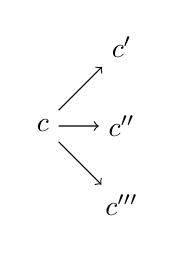
\begin{tikzpicture}[grow=right, ->, level distance=1cm,
            level 1/.style={sibling distance=1cm}]
            \node {$c$}
              child {node {$c'''$}}
              child {node {$c''$}}
              child {node {$c'$}};
        \end{tikzpicture}
    \end{center}    
\end{itemize}

\paragraph{Esempio: Reachability Problem} Dato un grafo diretto $G=(V,E)$, e due nodi $u,v\in V$, decidere se $u$ raggiunge $v$ (se esiste un cammino da $u$ a $v$). Studiamo la complessità in tempo e spazio di questo problema utilizzando sia un modello deterministico che nondeterministico.
\subparagraph{Modello deterministico} Un possibile algoritmo per risolvere questo problema è BFS$(G,u)$. Si costruisce un albero con radice $u$, e ad ogni livello si aggiungono i nodi raggiungibili in un passo. Utilizzando dei colori, alla fine della visita tutti i nodi visitati saranno neri, e quelli non raggiungibili grigi: è sufficiente controllare se $v$ è nero. Se $v$ è raggiungibile da $u$, allora $v$ sarà raggiunto da $u$ in un numero di passi $\leq |V|$. Quindi, la \textbf{complessità in tempo} è $O(|V|+|E|)$, ovvero lineare rispetto alla dimensione del grafo. Con una macchina di Turing:
\begin{center}
    \begin{tikzpicture}
        \draw (0,1) -- (7,1);
        \draw (0,1.5) -- (7,1.5);
        \foreach \x in {0.5,1} {
          \draw (\x,1) -- (\x,1.5);
        };
        \node[above] at (0.75,1) {$\rhd$};
        \node[above] at (3.75,1) {$\dots$};
        \draw [decorate,
            decoration = {brace,amplitude=5pt}] (1,1.6) -- (3.95,1.6);
        \node[above] at (2.5,1.75) {$G$};
        \draw [decorate,
            decoration = {brace,amplitude=5pt}] (4.05,1.6) -- (4.95,1.6);
        \node[above] at (4.5,1.75) {$u$};
        \draw [decorate,
            decoration = {brace,amplitude=5pt}] (5.05,1.6) -- (6,1.6);
        \node[above] at (5.5,1.75) {$v$};
        \draw [decorate,
            decoration = {brace,mirror,amplitude=5pt}] (1,.9) -- (6,.9);
        \node[below] at (3.5,.75) {$n$};

        \draw (0,-1) -- (7,-1);
        \draw (0,-.5) -- (7,-.5);
        \foreach \x in {0.5,1} {
          \draw (\x,-1) -- (\x,-.5);
        };
        \node[above] at (0.75,-1) {$\rhd$};
        \node[above] at (3.75,-1) {$\dots$};
        \draw [decorate,
            decoration = {brace,amplitude=5pt}] (1,-.4) -- (3.5,-.4);
        \node[above] at (2.25,-.25) {colori};

        \draw (0,-2.5) -- (7,-2.5);
        \draw (0,-2) -- (7,-2);
        \foreach \x in {0.5,1} {
          \draw (\x,-2.5) -- (\x,-2);
        };
        \node[above] at (0.75,-2.5) {$\rhd$};
        \node[above] at (3.75,-2.5) {$\dots$};
        \draw [decorate,
            decoration = {brace,amplitude=5pt}] (1,-1.9) -- (3,-1.9);
        \node[above] at (2,-1.75) {$Q$};
    \end{tikzpicture}
\end{center}
con $Q$ queue. Quindi, per la tesi di Church-Turing estesa, la complessità è $O(n^\alpha)$ per qualche $\alpha\in\mathbb{N}$. Si ha che
$$
    \text{Reachability} \in \text{P}
$$
Per quanto riguarda la \textbf{complessità in spazio}, si ha che i colori e $Q$ sono molto gradi, quindi
$$
    \text{Reachability} \in \text{PSPACE}
$$
\textbf{Esercizio}: migliorare questo risultato. In particolare, $\text{Reachability} \in \mathbb{L} = \text{SPACE}(\log n)$? $\text{Reachability} \in \text{SPACE}((\log n)^2)$?
\subparagraph{Modello nondeterministico} Si hanno diversi possibili stati futuri. Immaginiamo un grafo con un cammino da $u$ a $v$. Una macchina deterministica segue tutti i cammini uno ad uno, e per ognuno controlla se è quello corretto. Una macchina nondeterministica è in grado di ``indovinare'' il cammino corretto e di seguirlo.

Analizziamo la \textbf{complessità spaziale}. In questo caso non si ha bisogno dei colori. La macchina nondeterministica genera ad ogni passo un nuovo nodo nel working tape:
\begin{center}
    \begin{tikzpicture}
        \draw (0,1) -- (10.5,1);
        \draw (0,1.5) -- (10.5,1.5);
        \foreach \x in {0.5,1,2,2.5,3.5,4,5,5.5,6,7,7.5,8.5,9,10} {
          \draw (\x,1) -- (\x,1.5);
        };
        \node[above] at (0.75,1) {$\rhd$};
        \node[above] at (2.25,.9) {(};
        \node[above] at (3.75,1) {;};
        \node[above] at (5.25,.9) {)};
        \node[above] at (5.75,1) {;};
        \node[above] at (6.5,1) {$\dots$};
        \node[above] at (7.25,1) {;};
        \node[above] at (8.75,1) {;};
        \draw [decorate,
            decoration = {brace,amplitude=5pt}] (1,1.6) -- (2,1.6);
        \node[above] at (1.5,1.75) {$|V|$};
        \draw [decorate,
            decoration = {brace,amplitude=5pt}] (2.5,1.6) -- (3.5,1.6);
        \node[above] at (3,1.75) {$a$};
        \draw [decorate,
            decoration = {brace,amplitude=5pt}] (4,1.6) -- (5,1.6);
        \node[above] at (4.5,1.75) {$b$};
        \draw [decorate,
            decoration = {brace,amplitude=5pt}] (7.5,1.6) -- (8.5,1.6);
        \node[above] at (8,1.75) {$u$};
        \draw [decorate,
            decoration = {brace,amplitude=5pt}] (9,1.6) -- (10,1.6);
        \node[above] at (9.5,1.75) {$v$};
        \draw [decorate,
            decoration = {brace,mirror,amplitude=5pt}] (2,.9) -- (7,.9);
        \node[below] at (4.5,.75) {$\substack{\text{\normalsize archi}\\\text{\footnotesize worst case }O(|V|\cdot\log |V|)=n}$};
        \node[left] at (-.5,1.25) {input};

        \draw (0,-1) -- (10.5,-1);
        \draw (0,-.5) -- (10.5,-.5);
        \foreach \x in {0.5,1} {
          \draw (\x,-1) -- (\x,-.5);
        };
        \node[above] at (0.75,-1) {$\rhd$};
        \node[above] at (5,-1) {$\dots$};
        \node[ellipse,
            draw,
            minimum width=1.6cm,
            minimum height=.75cm] (A) at (1.75,-.75) { };
        \node[ellipse,
            draw,
            minimum width=1.6cm,
            minimum height=.75cm] (A) at (3.4,-.75) { };
        \node[below] at (1.75,-1.1) {$1.$};
        \node[below] at (3.4,-1.1) {$3.$};
        \node[left] at (-.3,-.75) {working t.};
    \end{tikzpicture}
\end{center}
\begin{enumerate}
    \item Genera il codice di un nodo (ad esempio, del nodo $a$)
    \item Controlla se esiste un arcp da $u$ ad $a$
    \begin{itemize}
        \item Se non esiste, ritorna ``no''
        \item Se esiste, vai avanti
    \end{itemize}
    \item Aggiungi un altro nodo (ad esempio, il nodo $b$)
    \item Controlla se esiste un arco da $a$ ad $b$
    \begin{itemize}
        \item Se non esiste, ritorna ``no''
        \item Se esiste, vai avanti
    \end{itemize}
    \item Sostituisci $a$ con $b$, e aggiungi un altro nodo (ad esempio, il nodo $c$)
    \item \dots
\end{enumerate}
\subparagraph{Esempio} Consideriamo il grafo
\begin{center}
    \begin{tikzpicture}[node distance={20mm}, main/.style = {}] 
        \node[main] (u) {$u$}; 
        \node[main] (a) [above right of=u] {$a$}; 
        \node[main] (b) [below right of=u] {$b$}; 
        \node[main] (c) [below left of=b] {$c$}; 
        \node[main] (d) [below right of=b] {$d$}; 
        \node[main] (e) [above right of=a] {$e$};
        \node[main] (f) [below right of=a] {$f$};
        \node[main] (v) [right of=f] {$v$}; 
        \draw[->] (u) -- (a);
        \draw[->] (a) -- (b);
        \draw[->] (b) -- (u);
        \draw[->] (d) -- (b);
        \draw[->] (b) -- (c);
        \draw[->] (c) -- (d);
        \draw[->] (a) -- (e);
        \draw[->] (a) -- (f);
        \draw[->] (f) -- (v);  
    \end{tikzpicture} 
\end{center}
Proviamo a trovare un cammino da $u$ a $v$:
\begin{itemize}
    \item Esiste un arco da $u$ ad $a$? Sì, quindi $ua$
    \item Esiste un arco da $a$ a $e$? Sì, quindi $uae$
    \item Esiste un arco da $e$ a $c$? No, quindi non esiste un cammino $uaec$
\end{itemize}
Esiste invece una computazione che genera il cammino $uafv$? Sì.
Si può notare come ci sia però un problema, ovvero i cicli (ad esempio $uabuabcdbcdb\dots$). In realtà, questo non è un problema: ragionando sulla complessità, e non sulla computabilità, consideriamo solo macchine di Turing che terminano.

Un modo per evitare i cicli è quello di immagazzinare in un working tape un contatore di passi eseguiti. Quando tale contatore raggiunge $|V|+1$, si può fermare la computazione e ritornare ``no''. 
$$
    \text{Reachability} \in \text{N}\mathbb{L} = \text{NSPACE}(\log n)
$$

\begin{definition}[Macchina Nondeterministica]
    Una macchina nondeterministica è una tupla $\mathcal{N}(K,\Sigma,\Delta,s)$, dove
    \begin{itemize}
        \item $K$ è un insieme finito di stati, di cui $s\in K$ è quello iniziale
        \item $\Sigma$ è un alfabeto finito, e $\rhd,\sqcup\in\Sigma$.
        \item $\Delta$ è la relazione di transizione, definita come 
        $$
        \Delta\subseteq K\times\Sigma^k\times (K\cup\{\text{yes},\text{no},\text{halt}\}) \times \Sigma^k \times \{\gets,\to,-\}^k
        $$
    \end{itemize}
    La relazione di transizione tra due configurazioni è definita come per le macchine deterministiche:
    $$
        (q,u_1,w_1,\dots,q_k,w_k) \to (q',u_1',w_1',\dots,q_k',w_k')
    $$
    con $(q',u_1',w_1',\dots,q_k',w_k')$ uno dei possibili risultati dell'applicazione di $\Delta$.
\end{definition}

\begin{definition}[Linguaggio deciso da una Macchina Nondeterministica]
    Un lin\-guag\-gio $L\subseteq(\Sigma\backslash\{\sqcup\})^*$ è deciso da una macchina nondeterministica $\mathcal{N}$ (con $\mathcal{N}(x)$ che termina sempre)
    \begin{itemize}
        \item[] se $\forall x\in L(\Sigma\backslash\{\sqcup\})^*$
        \begin{itemize}
            \item $x\in L$ $\Rightarrow$ esiste una computazione di $\mathcal{N}$ che inizia da $(s,\rhd,x,\rhd,\varepsilon,\dots,\rhd,\varepsilon)$ e termina in $(\text{yes},\dots)$
            \item $x\notin L$ $\Rightarrow$ tutte le computazioni di $\mathcal{N}$ che iniziano da $(s,\rhd,x,\rhd,\varepsilon,\dots,\rhd,\varepsilon)$ terminano in $(\text{no},\dots)$
        \end{itemize}
    \end{itemize}
\end{definition}
Se si ha una macchina che decide un linguaggio, bisogna definire la complessità spaziale e temporale su quella macchina. Per le macchine deterministiche, si ha che la complessità temporale è la lunghezza della computazione ne laso peggiore, per ogni possibile stringa di lunghezza $n$:
\begin{center}
    \begin{tikzpicture}[]
        \node (a1) at (0,0) {$\bullet$};
        \node (a2) at (0,-1) {$\bullet$};
        \node (a3) at (0,-2) {$\bullet$};
        \node (a4) at (0,-3) {$\bullet$};
        \node (b1) at (2,0) {$\bullet$};
        \node (b2) at (2,-1) {$\bullet$};
        \node (b3) at (2,-2) {$\bullet$};
        \node (b4) at (2,-3) {$\bullet$};
        \node (b5) at (2,-4) {$\bullet$};
        \node (b6) at (2,-5) {$\bullet$};
        \draw (a1) -- (a2) -- (a3) -- (a4);
        \draw (b1) -- (b2) -- (b3) -- (b4) --(b5) -- (b6);
        \node [above] at (a1) {$x\in L$};
        \node [left] at (a4) {yes};
        \node [above] at (b1) {$x\not\in L$};
        \node [right] at (b6) {no};
    \end{tikzpicture}
\end{center}
Ma nel caso nondeterministico si hanno degli alberi:
\begin{center}
    \begin{tikzpicture}[]
    \tikzstyle{level 1}=[sibling distance=4cm, level distance=1.2cm]
    \tikzstyle{level 2}=[sibling distance=1.6cm]
    \tikzstyle{level 3}=[sibling distance=1.6cm]
        \node (root) {$\bullet$}
        child {
            node (firstnode) {$\bullet$}
            child {
                node {no}        
                edge from parent 
            }
            child {
                node {$\bullet$}
                child {
                    node {$\bullet$}
                    child {
                        node {no}
                        edge from parent
                    }
                    child {
                        node {yes}
                        edge from parent
                    }
                    edge from parent
                }
                edge from parent 
            }        
            child {
                node {yes}
                edge from parent
            }
            edge from parent 
        }
        child {
            node {$\bullet$} 
            child {
                node {no}
                edge from parent
            }
            child {
                node {$\bullet$}
                child {
                    node {no}
                    edge from parent
                }
                child {
                    node {$\bullet$}
                    child {
                        node {no}
                        edge from parent
                    }
                    edge from parent
                }
                edge from parent         
            }
            edge from parent         
        }
        child {
            node {no}
            edge from parent
        };

    \node [above] at (root) {$x\in L$};
    \node [right] at (root.east) {$(s,\rhd,x,\dots)$};
    \node [left] at (firstnode) {$(q_1,w_1,\dots)$};
    \end{tikzpicture}
\end{center}

\begin{center}
    \begin{tikzpicture}[]
    \tikzstyle{level 1}=[sibling distance=4cm, level distance=1.2cm]
    \tikzstyle{level 2}=[sibling distance=1.6cm]
    \tikzstyle{level 3}=[sibling distance=1.6cm]
        \node (root) {$\bullet$}
        child {
            node (firstnode) {$\bullet$}
            child {
                node {no}        
                edge from parent 
            }
            child {
                node {$\bullet$}
                child {
                    node {$\bullet$}
                    child {
                        node {no}
                        edge from parent
                    }
                    child {
                        node {no}
                        edge from parent
                    }
                    edge from parent
                }
                edge from parent 
            }        
            child {
                node {no}
                edge from parent
            }
            edge from parent 
        }
        child {
            node {$\bullet$} 
            child {
                node {no}
                edge from parent
            }
            child {
                node {$\bullet$}
                child {
                    node {no}
                    edge from parent
                }
                child {
                    node {$\bullet$}
                    child {
                        node {no}
                        edge from parent
                    }
                    edge from parent
                }
                edge from parent         
            }
            edge from parent         
        }
        child {
            node {no}
            edge from parent
        };

    \node [above] at (root) {$x\not\in L$};
    \node [right] at (root.east) {$(s,\rhd,x,\dots)$};
    \node [left] at (firstnode) {$(q_1,w_1,\dots)$};
    \end{tikzpicture}
\end{center}
In questo caso, la complessità si può definire come l'altezza dell'albero.

\begin{definition}[Complessità Temporale di una Macchina Nondeterministica]
    U\-na macchina di Turing nondeterministica $\mathcal{N}$ con input $x$ richiede tempo $t$ se ogni possibile computazione di $\mathcal{N}$ su $x$ ha lunghezza al massimo $t$. 
    $\mathcal{N}$ richiede tempo $f(n)$ se, per ogni $x$, $\mathcal{N}$ termina su $x$ in tempo $f(|x|)$.
\end{definition}

\paragraph{Esempio} Immaginiamo che il grado del nondeterminismo di una macchina $\mathcal{N}$ sia 3, ovvero i nodi del suo albero hanno grado 3 ($d=3$). L'altezza è $f(|x|)$, e il numero di foglie è $d^{f(|x|)}$ (molto grande).


\begin{definition}[$\text{NTIME}(f(n))$]
    $L\in\text{NTIME}(f(n))$ se esiste una macchina di Turing nondeterministica $\mathcal{N}$ che decide $L$ in tempo $f(n)$.
\end{definition}
Notare che, ad esempio, $\text{TIME}(n^5)\neq\text{NTIME}(n^5)$. Quest'ultimo è l'insieme di tutti i linguaggi che possono essere decisi in tempo $n^5$ da una macchina di Turing nondeterministica.

\begin{proposition}
    $$
        \text{TIME}(f(n)) \subseteq \text{NTIME}(f(n))
    $$
\end{proposition}
Abbiamo che
$$
    \text{P} = \bigcup_{h\in\mathbb{N}} \text{TIME}(n^h)
    \qquad \qquad 
    \text{NP} = \bigcup_{h\in\mathbb{N}} \text{NTIME}(n^h)
$$
Quindi
$$
    \text{P} \subseteq \text{NP}
$$
Abbiamo definito la complessità temporale di una macchina nondeterministica. Possiamo definire anche la complessità spaziale come la configurazione (nodo dell'albero) massima.
\begin{definition}[Complessità Spaziale di una Macchina Nondeterministica]
    Una macchina di Turing nondeterministica con I/O $\mathcal{N}$ sull'input $x$ utilizza spazio $s$ se 
    $$
        s \geq \sum_{h=2}^{k-1} |w_h| + |u_h|
    $$
    Ovvero $s$ è il massimo su tutte le possibili computazioni di $\mathcal{N}$ su $x$
    $$
        s = \max\left( \sum |w_h| + |u_h| \right)
    $$
\end{definition}
$\mathcal{N}$ lavora in NSPACE$f(n)$, $\mathcal{N}$ decide $L$ in NSPACE$f(n)$.
\begin{align*}
    \text{PSPACE}=\mathbb{L} & ~\text{ spazio polinomiale su modello deterministico}\\
    \text{NPSPACE}=\text{N}\mathbb{L} & ~\text{ spazio polinomiale su modello nondeterministico} 
\end{align*}


% LEZIONE 14
\subsection{Simulazione di una Macchina Nondeterministica}
In una macchina di Turing nondeterministica si possono avere tre possibili casi durante la computazione:
\begin{enumerate}
    \item Si arriva ad una foglia con yes o no. In questo caso una macchina di Turing deterministica si comporta come
    \begin{center}
        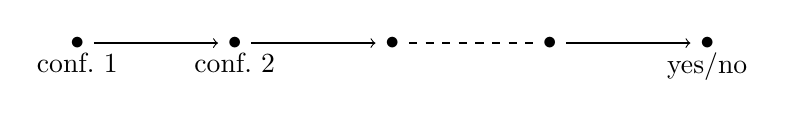
\begin{tikzpicture}
            \node (a) at (0,0) {$\bullet$};
            \node[below] at (a) {conf.~1};
            \node (b) at (2,0) {$\bullet$};
            \node[below] at (b) {conf.~2};
            \node (c) at (4,0) {$\bullet$};
            \node (d) at (6,0) {$\bullet$};
            \node (e) at (8,0) {$\bullet$};
            \node[below] at (e) {yes/no};
            \draw[->] (a) -- (b);
            \draw[->] (b) -- (c);
            \draw[dashed] (c) -- (d);
            \draw[->] (d) -- (e);
        \end{tikzpicture}
    \end{center}
    \item C'è un loop dal quale non si può uscire una volta entrati. In una macchina deterministica si ha
    \begin{center}
        \begin{tikzpicture}
            \node (a) at (0,0) {$\bullet$};
            \node (b) at (2,0) {$\bullet$};
            \node (c) at (4,0) {$\bullet$};
            \node (d) at (6,0) {$\bullet$};
            \node (e) at (8,0) {$\bullet$};
            \node (f) at (10,0) {$\bullet$};
            \node (g) at (12,0) {$\bullet$};
            \draw[->] (a) -- (b);
            \draw[->] (b) -- (c);
            \draw[dashed] (c) -- (d);
            \draw[->] (d) -- (e);
            \draw[->] (e) -- (f);
            \draw[->] (f) -- (g);
            \draw[->] (g) to [out=270,in=270,looseness=.5] (e);
        \end{tikzpicture}
    \end{center}
    \item Si ha un loop dal quale si può uscire. In una macchina deterministica si ha un cammino infinito che continua a cambiare configurazione
    \begin{center}
        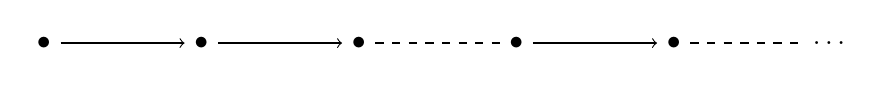
\begin{tikzpicture}
            \node (a) at (0,0) {$\bullet$};
            \node (b) at (2,0) {$\bullet$};
            \node (c) at (4,0) {$\bullet$};
            \node (d) at (6,0) {$\bullet$};
            \node (e) at (8,0) {$\bullet$};
            \node (f) at (10,0) {\dots};
            \draw[->] (a) -- (b);
            \draw[->] (b) -- (c);
            \draw[dashed] (c) -- (d);
            \draw[->] (d) -- (e);
            \draw[dashed] (e) -- (f);
        \end{tikzpicture}
    \end{center}
\end{enumerate}
Come già detto in precedenza, dato che questo è un corso sulla complessità, si considerano solo macchine di Turing che terminano sempre. Possiamo quindi procedere con la simulazione di una macchina non\-de\-ter\-ministica da parte di una macchina deterministica. Ricordiamo che, in una macchina di Turing nondeterministica $\mathcal{N}=(K,\Sigma,\Delta,s)$, $\Delta$ è la relazione di transizione
$$
    \Delta \subseteq \underbrace{K\times\Sigma^k}_{\substack{\text{input della}\\\text{relazione di}\\\text{transizione}}}\times (K\cup\{\text{yes},\text{no},\text{halt}\}) \times \Sigma^k \times \{\gets,\to,-\}^k
$$
\begin{definition}[Grado di nondeterminismo]
    Il grado di nondeterminismo di una macchina nondeterministica $\mathcal{N}$ è la ramificazione (il grado) massimo dell'albero di computazione di $\mathcal{N}$ per ogni $x\in\Sigma^*$.
    $$
        d(\mathcal{N}) = 
        \max_{\substack{q\in K\\\sigma_1,\dots,\sigma_k\in\Sigma}} 
        |\{ (q, \sigma_1, \dots, \sigma_k, q',\dots)\in\Delta \}|
    $$
\end{definition}
In particolare si ha
$$
    d(\mathcal{N})=1 ~\Leftrightarrow~ \mathcal{N} \text{ è deterministica}
$$
Consideriamo solo macchine con grado di nondeterminismo $d(\mathcal{N})\geq 2$. Sia $\mathcal{N}$ macchina con $d(\mathcal{N})=d$. $\mathcal{N}$ decide $L$ in tempo $f(n)$ (altezza dell'albero). Studiamo come la compessità temporale cambia restringendo il potere della macchina, ad esempio utilizzando $\mathcal{N}'$ con $d(\mathcal{N}')=2$.
\begin{itemize}
    \item In $\mathcal{N}$ l'altezza dell'albero è $f(n)$, e nel caso perggiore si hanno $d^{f(n)}$ foglie.
    \begin{center}
        \begin{tikzpicture}
            \node (a) {$\bullet$}
                child {node (b) {$\bullet$}}
                child {node (c) {$\bullet$}}
                child {node (d) {$\bullet$}}
                child {node (e) {$\bullet$}};
            \node[above] at (a) {a};
            \node[below] at (b) {b};
            \node[below] at (c) {c};
            \node[below] at (d) {d};
            \node[below] at (e) {e};
            \node at (0,-2.2) {$\vdots$};
        \end{tikzpicture}
    \end{center}
    \item In $\mathcal{N}'$ l'albero è del tipo 
    \begin{center}
        \begin{tikzpicture}
        \tikzstyle{level 1}=[sibling distance=2.5cm, level distance=1cm]
            \node (a) {$\bullet$}
                child {node (b) {$\bullet$}}
                child {node {$\bullet$}
                    child {node (c) {$\bullet$}}
                    child {node {$\bullet$}
                        child {node (d) {$\bullet$}}
                        child {node (e) {$\bullet$}}
                    }
                };
            \node[above] at (a) {a};
            \node[below] at (b) {b};
            \node[below] at (c) {c};
            \node[below] at (d) {d};
            \node[below] at (e) {e};
            \node at (0,-3.6) {$\vdots$};
        \end{tikzpicture}
    \end{center}
    In questo caso l'altezza dell'albero è $\log_2 (d^{f(n)}) = f(n)\log_2 (d)$, 
\end{itemize}
L'altezza cambia quindi solo di una costante, da $f(n)$ a $f(n)\log_2 (d)$.\medskip

Se proviamo a fare la stessa trasformazione utilizzando una macchina deterministica $\mathcal{M}$, la lunghezza è $(d')^{f(n)}$.
\begin{center}
    \begin{tikzpicture}
        \node (a) at (0,0) {$\bullet$};
        \node[above] at (a) {a};
        \node (b) at (2,0) {$\bullet$};
        \node (c) at (4,0) {$\bullet$};
        \node[above] at (c) {b$'$};
        \node[below] at (c) {$\LARGE\substack{\uparrow\\\text{no}\\\text{\footnotesize bisogna, ad es, fare backtracking}}$};
        \node (d) at (6,0) {$\bullet$};
        \node[above] at (d) {b$''$};
        \node (e) at (8,0) {$\bullet$};
        \node[above] at (e) {b$'''$};
        \node (f) at (10,0) {\dots};
        \draw[->] (a) -- (b);
        \draw[dashed] (b) -- (c);
        \draw[->] (c) -- (d);
        \draw[->] (d) -- (e);
        \draw[dashed] (e) -- (f);
    \end{tikzpicture}
\end{center}
\begin{theorem}
    Se $L$ è deciso da una macchina di Turing nondeterministica $\mathcal{N}$ in tempo $f(n)$, allora $L$ può essere deciso da una macchina di Turing deterministica $\mathcal{M}$ in tempo $O(c^{f(n)})$, con $c$ costante che dipende da $\mathcal{N}$.
\end{theorem}
\paragraph{Dimostrazione (intuizione)} La macchina $\mathcal{N}$ ha un input tape, una serie di working tape, e un output tape. La macchina $\mathcal{M}$ è costruita allo stesso modo, ma contiene un working tape in più. In ogni momento su questo nastro vengono registrate le scelte fatte dalla macchina $\mathcal{N}$. Ad esempio:
\begin{center}
    \begin{tikzpicture}
        % Draw the horizontal strip
        \draw (0,0) -- (4,0);
        \draw (0,.5) -- (4,.5);
        %  Draw the squares
        \foreach \x in {0.5,1,1.5} {
          \draw (\x,0) -- (\x,.5);
        };
        \node[above] at (0.75,0) {$\rhd$};
        \node[above] at (1.25,0) {$1$};
        \node[below] at (1.25,0) {$c_1$};
        \node[above] at (2.5,0) {\dots};
    \end{tikzpicture}
\end{center}
L'1 significa che viene preso il primo ramo dell'albero: viene simulata $\mathcal{N}$ con, come prima scelta, $c_1$.
\begin{itemize}
    \item Se $\mathcal{N}$ termina con yes, $\mathcal{M}$ termina con yes
    \item Se $\mathcal{N}$ termina con no, $c_1$ viene incrementato (di 1) e si procede nella simulazione 
    \item Se $\mathcal{N}$ non termina, si genara $c_2=1$
    \begin{center}
        \begin{tikzpicture}
            % Draw the horizontal strip
            \draw (0,0) -- (4,0);
            \draw (0,.5) -- (4,.5);
            %  Draw the squares
            \foreach \x in {0.5,1,1.5,2} {
              \draw (\x,0) -- (\x,.5);
            };
            \node[above] at (0.75,0) {$\rhd$};
            % \node[above] at (1.25,0) {$1$};
            \node[below] at (1.25,0) {$c_1$};
            \node[above] at (1.75,0) {$1$};
            \node[below] at (1.75,0) {$c_2$};
            \node[above] at (3,0) {\dots};
        \end{tikzpicture}
    \end{center}
\end{itemize}
Il cammino più a sinistra di $\mathcal{N}$ sarà
\begin{center}
    \begin{tikzpicture}
        % Draw the horizontal strip
        \draw (0,0) -- (5,0);
        \draw (0,.5) -- (5,.5);
        %  Draw the squares
        \foreach \x in {0.5,1,1.5,,2,4,4.5} {
          \draw (\x,0) -- (\x,.5);
        };
        \node[above] at (0.75,0) {$\rhd$};
        \node[above] at (1.25,0) {$1$};
        \node[above] at (1.75,0) {$1$};
        \node[above] at (3,0) {\dots};
        \node[above] at (4.25,0) {$1$};
        \draw[decorate,
            decoration = {brace,mirror,amplitude=5pt}] (1,-0.1) -- (4.5,-0.1);
        \node[below] at (2.75,-.2) {$O(f(n))$};
    \end{tikzpicture}
\end{center}
Se ci si trova in un caso in cui vengono percorsi tutti i rami uscenti da un nodo senza arrivare ad una soluzione yes, ad esempio
\begin{center}
    \begin{tikzpicture}
        % Draw the horizontal strip
        \draw (0,0) -- (5,0);
        \draw (0,.5) -- (5,.5);
        %  Draw the squares
        \foreach \x in {0.5,1,1.5,,2,3,3.5,4} {
          \draw (\x,0) -- (\x,.5);
        };
        \node[above] at (0.75,0) {$\rhd$};
        \node[above] at (1.25,0) {$1$};
        \node[above] at (1.75,0) {$1$};
        \node[above] at (2.5,0) {\dots};
        \node[above] at (3.25,0) {$1$};
        \node[above] at (3.75,0) {$d$};
        \node[above] at (4.5,0) {\dots};
    \end{tikzpicture}
\end{center}
si farà backtracking:
\begin{center}
    \begin{tikzpicture}
        % Draw the horizontal strip
        \draw (0,0) -- (5,0);
        \draw (0,.5) -- (5,.5);
        %  Draw the squares
        \foreach \x in {0.5,1,1.5,,2,3,3.5,4} {
          \draw (\x,0) -- (\x,.5);
        };
        \node[above] at (0.75,0) {$\rhd$};
        \node[above] at (1.25,0) {$1$};
        \node[above] at (1.75,0) {$1$};
        \node[above] at (2.5,0) {\dots};
        \node[above] (b) at (3.25,0) {$2$};
        \node[above] (a) at (3.75,0) {$d$};
        \node[above] at (4.5,0) {\dots};

        \draw[->] (a) to [out=270,in=270,looseness=2.5] (b);

        \draw (0,-1) -- (5,-1);
        \draw (0,-1.5) -- (5,-1.5);
        %  Draw the squares
        \foreach \x in {0.5,1,1.5,,2,3,3.5,4} {
          \draw (\x,-1.5) -- (\x,-1);
        };
        \node[above] at (0.75,-1.5) {$\rhd$};
        \node[above] at (1.25,-1.5) {$1$};
        \node[above] at (1.75,-1.5) {$1$};
        \node[above] at (2.5,-1.5) {\dots};
        \node[above] (c) at (3.25,-1.5) {$2$};
        \node[above] (d) at (3.75,-1.5) {$1$};
        \node[above] at (4.5,-1.5) {\dots};

        \draw[->] (c) to [out=270,in=270,looseness=2.5] (d);
    \end{tikzpicture}
\end{center}
Se ogni cammino finisce con no, si avrà
\begin{center}
    \begin{tikzpicture}
        % Draw the horizontal strip
        \draw (0,0) -- (5,0);
        \draw (0,.5) -- (5,.5);
        %  Draw the squares
        \foreach \x in {0.5,1,1.5,,2,4,4.5} {
          \draw (\x,0) -- (\x,.5);
        };
        \node[above] at (0.75,0) {$\rhd$};
        \node[above] at (1.25,0) {$d$};
        \node[above] at (1.75,0) {$d$};
        \node[above] at (3,0) {\dots};
        \node[above] at (4.25,0) {$d$};
        \draw[decorate,
            decoration = {brace,mirror,amplitude=5pt}] (1,-0.1) -- (4.5,-0.1);
        \node[below] at (2.75,-.2) {$O(f(n))$};
    \end{tikzpicture}
\end{center}
che corrisponde all'ultimo cammino nell'albero.

Per generare uno dei bit della sequenza (che vogliamo simulare) di scelte, $\mathcal{M}$ utilizza un numero di passi pari a $O\left(f(n)\cdot\log_2(d)\right)$. Quindi, per generarli tutti, si ha
$$
    O\left(d^{f(n)}\cdot f(n)\cdot\log_2(d)\right)
$$
I passi di simulazione di $\mathcal{N}$ sono 
$$
    O\left(d^{f(n)}\right)
$$
Unendo tutto, abbiamo che
$$
    O\left(d^{f(n)} + d^{f(n)}\cdot f(n)\cdot\log_2(d)\right)= 
    O\left(d^{f(n)}\cdot 2^{f(n)}\right)=
    O\left(c^{f(n)}\right)
$$
Notiamo come questa simulazione può essere fatta senza conoscere $f(n)$. \hfill $\square$

\begin{corollary}
    $$
        \text{NP} \subseteq \text{EXP}
    $$
\end{corollary}
\paragraph{Dimostrazione} $\mathcal{N}$ decide $L$ in tempo $n^h$. $\mathcal{N}$ può essere simulata da una macchina deterministica $\mathcal{M}$ in tempo 
$$
    O\left(c^{n^h}\right) =
    O\left(2^{\log_2c\cdot n^h}\right) =
    O\left(2^{n^{h+1}}\right)
$$
che è incluso nella classe EXP. \hfill $\square$

\subparagraph{Nota} $O(c^{n^h})$ non è dello stesso ordine di $\Theta(2^{n^h})$.



\chapter{Relazioni tra Classi di Complessità}

Capitolo 7 del libro di Papadimitriou. Finora abbiamo visto:
\begin{enumerate}
    \item \textbf{Modelli di computazione}: macchine di Turing
    \item \textbf{Modi di computazione}: deterministico, nondeterministico
    \item \textbf{Risorse}: tempo, spazio
    \item \textbf{Funzioni utilizzate come limiti}, ad esempio TIME$f(n)$, SPACE$f(n)$
\end{enumerate}
In questo capitolo vedremo meglio il punto 4, e inoltre
\begin{itemize}
    \item \textbf{Funzioni di complessità proprie} 
    \item Due risultati fondamentali:
    \begin{itemize}
        \item \textbf{Hierarchy Theorem}, ovvero se $f$ è propria, allora $\text{TIME}(f(n))\subsetneq \text{TIME}(f(n)^3)$. Esiste una gerarchia propria tra classi che sono tutte non uguali tra loro;
        \item \textbf{Gap Theorem}, ovvero che esiste $f$ non propria tale che $\text{TIME}(f(n))=\text{TIME}(2^{f(n)})$.
    \end{itemize}
\end{itemize}


\section{Classi di Complessità}

\begin{definition}[Funzione di Complessità Propria]
    Una funzione $f:\mathbb{N}\to\mathbb{N}$ è una funzione di complessità propria se
    \begin{enumerate}
        \item $f$ è non decrescente
        \item Esiste $\mathcal{M}_f$ macchina di Turing deterministica con I/O tale che, per ogni $x$ con $|x|=n$ 
        $$
            (s, \rhd, x, \rhd, \varepsilon, \dots, \rhd, \varepsilon) 
            \to^{(\mathcal{M}_f)t} 
            (h, 
            \underbrace{u,w}_{\rhd x\sqcup}, 
            \underbrace{\rhd,\sqcup^{j_2},\dots,\rhd,\sqcup^{j_{k-1}}}_{\text{working tapes}}, 
            \underbrace{\rhd,\sqcap^{f(x)}}_{\text{output tape}})
        $$
        con $\sqcap^{f(x)}$ rappresentazione unaria di $f(x)$. Inoltre,
        \begin{itemize}
            \item $t\in O(n+f(n))$
            \item $j_2,\dots,j_{k-1}\in O(f(n))$
            \item $t,j_2,\dots,j_{k-1}$ non dipendono da $x$
        \end{itemize}
    \end{enumerate}
\end{definition}
\paragraph{Nota} In $t\in O(n+f(n))$, bisogna aggiungere $n$ perché altrimenti non si potrebbe avere $\log(n)$ come funzione propria (bisogna leggere $n$).

\paragraph{Esempio} Si ha $\mathcal{M}_f$
\begin{center}
    \begin{tikzpicture}
        \draw (0,2) -- (5,2);
        \draw (0,2.5) -- (5,2.5);
        \foreach \x in {0.5,1,1.5,3.5,4,4.5} {
          \draw (\x,2) -- (\x,2.5);
        };
        \node[above] at (0.75,2) {$\rhd$};
        \node[above] at (1.25,2) {$x_1$};
        \node[above] at (2.5,2) {\dots};
        \node[above] at (3.75,2) {$x_n$};
        \node[above] at (4.25,2) {$\sqcup$};
        \draw[decorate,
            decoration = {brace,amplitude=5pt}] (1,2.6) -- (4,2.6);
        \node[above] at (2.5,2.7) {$n$};

        \draw (0,.75) -- (5,.75);
        \draw (0,1.25) -- (5,1.25);
        \foreach \x in {0.5,1,1.5,2,3.5,4,4.5} {
          \draw (\x,.75) -- (\x,1.25);
        };
        \node[above] at (0.75,.75) {$\rhd$};
        \node[below] at (0.65,.85) {$\uparrow$};
        \node[above] at (1.25,.75) {$\cancel{~~}$};
        \node[above] at (1.25,1.25) {$\sqcup$};
        \node[above] at (1.75,.75) {$\cancel{~~}$};
        \node[above] at (1.75,1.25) {$\sqcup$};
        \node[above] at (2.75,.75) {\dots};
        \node[above] at (3.75,.75) {$\cancel{~~}$};
        \node[above] at (3.75,1.25) {$\sqcup$};
        % \node[above] at (4.25,.75) {$\sqcup$};
        \draw[->] (3.7,.75) to [out=270,in=270,looseness=2] (3.3,.75);
        \draw[->] (2.2,.75) to [out=270,in=270,looseness=2] (1.8,.75);
        \draw[->] (1.7,.75) to [out=270,in=270,looseness=2] (1.3,.75);
        \draw[->] (1.2,.75) to [out=270,in=270,looseness=2] (0.8,.75);

        \node at (2,.15) {$\vdots$};
        \draw[decorate,
            decoration = {brace,amplitude=5pt}] (-.5,-.2) -- (-.5,1.6);
        \node[left] at (-.6,.7) {w.t.};

        \draw (0,-.5) -- (5,-.5);
        \draw (0,-1) -- (5,-1);
        \foreach \x in {0.5,1,1.5,3.5,4,4.5} {
          \draw (\x,-.5) -- (\x,-1);
        };
        \node[above] at (0.75,-1) {$\rhd$};
        \node[above] at (1.25,-1) {$\sqcap$};
        \node[above] at (2.5,-1) {\dots};
        \node[above] at (3.75,-1) {$\sqcap$};
        \node[above] at (4.25,-1) {$\sqcup$};
        \draw[decorate,
            decoration = {brace,mirror,amplitude=5pt}] (1,-1.1) -- (4,-1.1);
        \node[below] at (2.5,-1.2) {$f(n)$};
    \end{tikzpicture}
\end{center}
Su ogni working tape, viene eliminato tutto e si ferma a $\rhd$. Lo spazio utilizzato in tutti i working tape è $O(f(n))$.


% LEZIONE 15
\paragraph{Esempi di funzioni proprie}
\begin{align*}
    p(n) & \text{ polinomio} \\
    \log(n) & \text{ logaritmo} \\
    c & \text{ costante} \\
    2^{p(n)} & \text{ esponenziale} \\
    2^{2^{\rdots^{2^{p(n)}}}} & \text{ torre di esponenziali}
\end{align*}
La composizione di funzioni proprie è propria.

\begin{definition}[Macchine di Turing Precise]
    Una macchina di Turing con I/O $\mathcal{M}$ è precisa se $\exists f,g$ tali che $\forall x \in \Sigma^*$, $\mathcal{M}$ su $x$ termina in tempo $f(|x|)$ e utilizza spazio $g(|x|)$.
\end{definition}
Ad esempio, merge sort è preciso, mentre heap sort non lo è.

\begin{theorem}
    \begin{eqnarray*}
        & L \text{ è decidibile in TIME$(f(n))$ e $f$ è propria} &\\
        &\Downarrow& \\
        & \exists \text{ una macchina di Turing precisa $\mathcal{M}$ che decide $L$ in tempo }O(f(n)) &
    \end{eqnarray*}
\end{theorem}
\paragraph{Dimostrazione (idea)} (errore nel libro, proposizione 7.1.: macchina precisa in TIME e non in SPA\-CE) Sappiamo che se $L\in$TIME$(f(n))$, allora $\mathcal{M}$ decide $L$ in $f(n)$ passi. Se $f$ è propria, $\mathcal{M}_f$ computa $f(n)$.
\begin{center}
    \begin{tikzpicture}
        \node at (-.9,2.7) {$\mathcal{M}'$};
        \draw (0,2) -- (5,2);
        \draw (0,2.5) -- (5,2.5);
        \foreach \x in {0.5,1,1.5,3.5,4,4.5} {
          \draw (\x,2) -- (\x,2.5);
        };
        \node[above] at (0.75,2) {$\rhd$};
        \node[above] at (1.25,2) {$x_1$};
        \node[above] at (2.5,2) {\dots};
        \node[above] at (3.75,2) {$x_n$};
        \node[above] at (4.25,2) {$\sqcup$};

        \node at (2.5,1.3) {$\vdots$};

        \draw (0,.1) -- (5,.1);
        \draw (0,.6) -- (5,.6);
        \foreach \x in {0.5,1,1.5,3.5,4} {
          \draw (\x,.1) -- (\x,.6);
        };
        \node[above] at (0.75,.1) {$\rhd$};
        \node[above] at (1.25,.1) {$\sqcap$};
        \node[above] at (2.5,.1) {\dots};
        \node[above] at (3.75,.1) {$\sqcap$};
        \node[left] at (-.1,.35) {$\substack{\text{rappresentazione}\\\text{unaria di }f(n)}$};

        \draw (0,-.5) -- (5,-.5);
        \draw (0,-1) -- (5,-1);
        \foreach \x in {0.5,1} {
          \draw (\x,-.5) -- (\x,-1);
        };
        \node[above] at (0.75,-1) {$\rhd$};
        \node[above] at (2.5,-1) {\dots};

        \draw[decorate,
            decoration = {brace,mirror,amplitude=5pt}] (5.5,.9) -- (5.5,2.6);
        \node[right] at (5.6,1.8) {\Large$\substack{\text{tutti i nastri}\\\text{di }\mathcal{M}}$};
        \draw[decorate,
            decoration = {brace,mirror,amplitude=5pt}] (5.5,-1.1) -- (5.5,.7);
        \node[right] at (5.6,-.2) {$\mathcal{M}_f$};
    \end{tikzpicture}
\end{center}
~\hfill $\square$


\subsection{Classi di Complessità Complemento}
Una classe di complessità è un insieme di linguaggi (problemi) che possono essere decisi in un certo tempo, o spazio. Un linguaggio $L\subseteq \Sigma^*$ è un insieme di stringhe. Il complemento di $L$ è definito come
$$
    \overline{L} = \{ x ~|~ x\notin L \}
$$
\begin{definition}[Complemento di una Classe di Complessità, co-$\mathcal{C}$]
    Data una classe di complessità $C$, il complemento di $C$ è
    $$
        \text{co-}\mathcal{C} = \{ \overline{L} ~|~ L\in C \}
    $$
\end{definition}
\paragraph{Nota} $\text{co-}\mathcal{C} \neq \overline{\mathcal{C}}$ (= complemento di tutte le classi $\mathcal{C}$). \medskip

Se $\mathcal{C}$ è deterministica (si utilizza una macchina deterministica), e $\Sigma=\{0,1\}$, quando si prende un linguaggio appartenente a quella classe, ad esempio $L\in\text{TIME}(n\log n)$, allora esiste $\mathcal{M}$ macchina deterministica che decide $L$ in tempo $n\log n$.

Per ottenere $\overline{L}$ si possono scambiare yes e no, e la macchina ``complemento $\mathcal{M}$'' decide $\overline{L}\in\text{TIME}(n\log n)$. Questo vale per tutte le classi deterministiche.
\begin{property}
    $$
    \mathcal{C} \text{ è una classe di complessità deterministica }
    \Rightarrow
    ~\mathcal{C} = \text{co-}\mathcal{C}
    $$
\end{property}
\begin{property}
    Quando $\mathcal{C}$ è una classe di complessità deterministica
    $$
        L\in\mathcal{C} 
        ~\Rightarrow~
        \overline{L}\in\mathcal{C}
        ~\Rightarrow~
        \text{co-}\mathcal{C}\subseteq\mathcal{C}
    $$
\end{property}
Cosa succede se $\mathcal{C}$ è una classe di complessità nondeterministica?
\paragraph{Esempio} Consideriamo $\text{NP}=\bigcup_{h\in\mathbb{N}}\text{NTIME}(n^h)$. Se $L\in\text{NP}$, allora esiste $\mathcal{N}$ macchina nondeterministica che decide $L$.
\begin{itemize}
    \item Se $x\in L$, allora esiste un cammino nell'albero di computazione di $\mathcal{N}$ che arriva a yes.
    \item Se $x\notin L$, allora tutti i cammini nell'albero di computazione di $\mathcal{N}$ arrivano a no.
\end{itemize}
Consideriamo $\mathcal{N}'$ in cui le risposte di $\mathcal{N}$ sono invertite, che decide il linguaggio $L'$. Nel caso in cui $x\in L$, non è vero che $x\in L'$. Nell'albero di $\mathcal{N}'$ otteniamo alcuni yes non voluti, e quindi decide un linguaggio più ampio di $\overline{L}$. Quindi $\mathcal{N}'$ decide $L'$ con $L'\subseteq\overline{L}$.

\paragraph{Satisfiability Problem} Iniziamo con un esempio. Consideriamo la formula booleana 
$$
    \varphi = (p\lor\lnot q)\land(r\lor\lnot p)
$$
Quando si fissa una valutazione $v\{p,q,r\}\to\{0,1\}$, si può calcolare il valore di $\varphi$ con $v$. Ad esempio, se $v(p)=1$, $v(q)=0$, $v(r)=0$, allora $\varphi[v]=0$.

\begin{proposition}[Problema di Soddisfacibilità]
    Data una formula booleana $\varphi$, decidere se esiste $v:Var(\varphi)\to\{0,1\}$ tale che $\varphi[v]=1$.
\end{proposition}
In altre parole si vuole trovare il linguaggio
$$
    L = \{\varphi ~|~ \varphi \text{ è soddisfacibile}\}
$$
Studiamone la complessità. Una macchina nondeterministica efficiente per $L$ è:
\begin{itemize}
    \item In input si ha la formula 
    \begin{center}
        \begin{tikzpicture}
            \node[left] at (-.3,2.25) {input};
            \draw (0,2) -- (6.5,2);
            \draw (0,2.5) -- (6.5,2.5);
            \foreach \x in {0.5,1,...,6} {
              \draw (\x,2) -- (\x,2.5);
            };
            \node[above] at (0.75,2) {$\rhd$};
            \node[above] at (1.25,2) {$p$};
            \node[above] at (1.75,2) {$\lor$};
            \node[above] at (2.25,2) {$\lnot$};
            \node[above] at (2.75,2) {$q$};
            \node[above] at (3.25,2) {$\land$};
            \node[above] at (3.75,2) {$r$};
            \node[above] at (4.25,2) {$\lor$};
            \node[above] at (4.75,2) {$\lnot$};
            \node[above] at (5.25,2) {$p$};
            \node[above] at (5.75,2) {$\sqcup$};
        \end{tikzpicture}
    \end{center}
    \item Scansionare l'input per contare le variabili
    \begin{center}
        \begin{tikzpicture}
            \node[left] at (-.3,2.25) {w.t.~1};
            \draw (0,2) -- (3,2);
            \draw (0,2.5) -- (3,2.5);
            \foreach \x in {0.5,1,1.5,2,2.5} {
              \draw (\x,2) -- (\x,2.5);
            };
            \node[above] at (0.75,2) {$\rhd$};
            \node[above] at (1.25,2) {$p$};
            \node[above] at (1.75,2) {$q$};
            \node[above] at (2.25,2) {$r$};
        \end{tikzpicture}
    \end{center}
    \item Generare nondeterministicamente un assegnamento
    \begin{center}
        \begin{tikzpicture}
            \node[left] at (-.3,2.25) {w.t.~2};
            \draw (0,2) -- (3,2);
            \draw (0,2.5) -- (3,2.5);
            \foreach \x in {0.5,1,1.5,2,2.5} {
              \draw (\x,2) -- (\x,2.5);
            };
            \node[above] at (0.75,2) {$\rhd$};
            \node[above] at (1.25,2) {0};
            \node[above] at (1.75,2) {0};
            \node[above] at (2.25,2) {0};
        \end{tikzpicture}
    \end{center}
    \item Controllare il valore di verità di tale assegnamento
    \begin{center}
        \begin{tikzpicture}[level distance=1.5cm,
            level 1/.style={sibling distance=6cm},
            level 2/.style={sibling distance=3cm},
            level 3/.style={sibling distance=1.5cm},
            level 4/.style={sibling distance=0.75cm}]
            \node at (-6.5,-.75) {$p$};
            \node at (-6.5,-2.25) {$q$};
            \node at (-6.5,-3.75) {$r$};
            \node (root) {$\bullet$}
              child {node {$\bullet$}
                child {node {$\bullet$}
                  child {node (yes) {$\bullet$}
                    edge from parent node[left] {0}
                  }
                  child {node {$\bullet$}
                    edge from parent node[right] {1}
                  }
                  edge from parent node[left] {0}
                }
                child {node {$\bullet$}
                  child {node {$\bullet$}
                    edge from parent node[left] {0}
                  }
                  child {node {$\bullet$}
                    edge from parent node[right] {1}
                  }
                  edge from parent node[right] {1}
                }
                edge from parent node[left] {0}
              }
              child {node {$\bullet$}
                child {node {$\bullet$}
                  child {node (no) {$\bullet$}
                    edge from parent node[left] {0}
                  }
                  child {node {$\bullet$}
                    edge from parent node[right] {1}
                  }
                  edge from parent node[left] {0}
                }
                child {node {$\bullet$}
                  child {node {$\bullet$}
                    edge from parent node[left] {0}
                  }
                  child {node {$\bullet$}
                    edge from parent node[right] {1}
                  }
                  edge from parent node[right] {1}
                }
                edge from parent node[right] {1}
              };
            \node[above] at (root) {$\mathcal{N}(\varphi)$};
            \node[below] at (yes) {yes};
            \node[below] at (no) {no};
        \end{tikzpicture}
    \end{center}
\end{itemize} 
Quindi SAT $\in$ NP.

\paragraph{Unsatisfiability Problem} Cosa succede per $\overline{L}$?
\begin{proposition}[Problema di Insoddisfacibilità]
    Data una formula booleana $\varphi$, decidere se per ogni $v:Var(\varphi)\to\{0,1\}$ si ha $\varphi[v]=0$.
\end{proposition}
In altre parole si vuole trovare il linguaggio
$$
    \overline{L} = \{\varphi ~|~ \varphi \text{ non è una formula, o \underline{è insoddisfacibile}}\}
$$
Controllare che $\varphi$ sia o meno una formula è banale, quindi ci concentriamo sulla sua insoddisfacibilità. Se scambiamo yes e no nelle foglie dell'albero di computazione, otteniamo questo:
\begin{center}
    \begin{tikzpicture}[level distance=1.5cm,
        level 1/.style={sibling distance=6cm},
        level 2/.style={sibling distance=3cm},
        level 3/.style={sibling distance=1.5cm},
        level 4/.style={sibling distance=0.75cm}]
        \node at (-6.5,-.75) {$p$};
        \node at (-6.5,-2.25) {$q$};
        \node at (-6.5,-3.75) {$r$};
        \node (root) {$\bullet$}
          child {node {$\bullet$}
            child {node {$\bullet$}
              child {node (yes) {$\bullet$}
                edge from parent node[left] {0}
              }
              child {node {$\bullet$}
                edge from parent node[right] {1}
              }
              edge from parent node[left] {0}
            }
            child {node {$\bullet$}
              child {node {$\bullet$}
                edge from parent node[left] {0}
              }
              child {node {$\bullet$}
                edge from parent node[right] {1}
              }
              edge from parent node[right] {1}
            }
            edge from parent node[left] {0}
          }
          child {node {$\bullet$}
            child {node {$\bullet$}
              child {node (no) {$\bullet$}
                edge from parent node[left] {0}
              }
              child {node {$\bullet$}
                edge from parent node[right] {1}
              }
              edge from parent node[left] {0}
            }
            child {node {$\bullet$}
              child {node {$\bullet$}
                edge from parent node[left] {0}
              }
              child {node {$\bullet$}
                edge from parent node[right] {1}
              }
              edge from parent node[right] {1}
            }
            edge from parent node[right] {1}
          };
        \node[above] at (root) {$\mathcal{N}'(\varphi)$};
        \node[below] at (yes) {no};
        \node[below] at (no) {yes};
    \end{tikzpicture}
\end{center}
$\mathcal{N}'$ accetta $\varphi$, ma $\varphi$ non è insoddisfacibile. $\mathcal{N}'$ non decide $\overline{L}$. Quindi UnSAT $\in$ co-NP.\medskip

Per il momento non conosciamo la relazione tra NP e co-NP.
$$
    \text{NP } ? \text{ co-NP}
$$
Decidere unSAT ha la stessa complessità di decidere Validity, quindi Validity $\in$ co-NP.



\section{Hierarchy Theorem}
Utilizzeremo il teorema per dire che esiste un numero infinito di classi di compessità diverse tra loro, ognuna propriamente contenuta dentro l'altra.

\begin{theorem}[Hierarchy Theorem]
    $$
        f \text{ è propria}
        ~\Rightarrow~
        \text{TIME}(f(n)) \subsetneq \text{TIME}(f(n)^3)
    $$
\end{theorem}
\paragraph{Dimostrazione} Versione quantitativa della dimostrazione dell'Halting Theorem (Capitolo 3 del libro).

\begin{theorem}[Halting Theorem]
    Il linguaggio
    $$
        H = \{ \mathcal{M};x ~|~ \mathcal{M}(x)\neq\uparrow \}
    $$
    è ricorsivamente enumerabile, ma non ricorsivo.
\end{theorem}
\paragraph{Dimostrazione (intuizione)} Si costruisce una macchina universale $\mathcal{U}$ che riceve in input la rappresentazione binaria della macchina $\mathcal{M}$ e della stringa $x$, e simula $\mathcal{M}$ su $x$. Ci sarà un working tape che contiene la configurazione di $\mathcal{M}$. Si può dimostrare che non si può modificare $\mathcal{U}$ in modo da dimostrare se $\mathcal{M}$ termina o meno su $x$ (Se $\mathcal{M}$ termina su $x$, $\mathcal{U}$ accetta; se $\mathcal{M}$ non termina su $x$, $\mathcal{U}$ non termina). 

Aggiungeremo un limite al numero di passi che si possono fare, dando quindi un risultato quantitativo.



% LEZIONE 16
\subsection{Dimostrazione dello Hierarchy Theorem}
Consideriamo il linguaggio 
$$
    H_f = \{ \mathcal{M};x ~|~ \mathcal{M} \text{ accetta $x$ in al massimo } f(|x|)+5|x|+4 \text{ passi}  \}
$$
Inoltre $\mathcal{M}(x)\downarrow$, e $\mathcal{M}(x)=$ yes. Per lo Hierarchy Theorem, $f$ è propria, e 
$$
    H_f\in\text{TIME}\left(f(2n+1)^3\right)
    \qquad \qquad
    H_f\notin\text{TIME}(f(n))
$$
Queste due classi di complessità sono diverse e sono una contenuta nell'altra. 
\begin{center}
    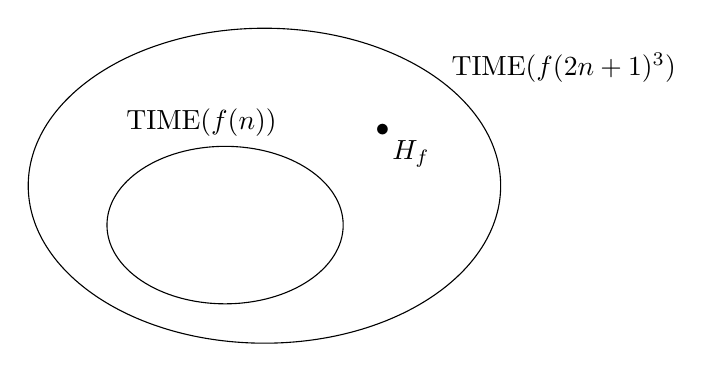
\begin{tikzpicture}
        % Outer ellipse representing TIME(f(2n+1)^3)
        \draw (0,0) ellipse (3cm and 2cm);
        \node at (3.8,1.5) {TIME$(f(2n+1)^3)$};
        
        % Inner ellipse representing TIME(f(n))
        \draw (-.5,-.5) ellipse (1.5cm and 1cm);
        \node at (-.8,.8) {TIME$(f(n))$};
      
        % Point representing H_f
        \node (h) at (1.5,0.7) {$\bullet$};
        \node[below right] at (h) {$H_f$};
    \end{tikzpicture}
\end{center}
Quindi
$$
    \text{TIME}(f(n)) \subsetneq \text{TIME}\left(f(2n+1)^3\right)
$$

\begin{lemma}
    $$
        H_f \in \text{TIME}(f(n)^3)
    $$
\end{lemma}
\paragraph{Dimostrazione} Si costruisce una macchina universale $\mathcal{U}_f$. Se $f$ è una funzione propria, allora anche la funzione $g(n)=f(n)+5n+4$ è propria.
\begin{center}
    \begin{tikzpicture}
        \draw (0,3.5) -- (7,3.5);
        \draw (0,4) -- (7,4);
        \foreach \x in {0.5,1,4,4.5,6.5} {
          \draw (\x,3.5) -- (\x,4);
        };
        \node[above] at (0.75,3.5) {$\rhd$};
        \node[above] at (4.25,3.5) {;};
        % \node[above] at (2.5,2) {\dots};
        % \node[above] at (3.75,2) {$x_n$};
        % \node[above] at (4.25,2) {$\sqcup$};
        \draw[decorate,
            decoration = {brace,amplitude=5pt}] (1,4.2) -- (4,4.2);
        \node[above] at (2.5,4.3) {$\mathcal{M}$};
        \draw[decorate,
            decoration = {brace,amplitude=5pt}] (4.5,4.2) -- (6.5,4.2);
        \node[above] at (5.5,4.3) {$x$};
        \draw[decorate,
            decoration = {brace,amplitude=5pt}] (1,4.9) -- (6.5,4.9);
        \node[above] at (3.75,5) {$n$};

        \draw (0,2) -- (7,2);
        \draw (0,2.5) -- (7,2.5);
        \foreach \x in {0.5,1,1.5,2.5,3,3.5} {
          \draw (\x,2) -- (\x,2.5);
        };
        \node[above] at (0.75,2) {$\rhd$};
        \node[above] at (1.25,2) {$x_1$};
        \node[above] at (2,2) {\dots};
        \node[above] at (2.75,2) {$x_n$};
        \node[above] at (3.25,2) {$\sqcup$};
        \draw[decorate,
            decoration = {brace,amplitude=5pt}] (1,2.7) -- (3,2.7);
        \node[above] at (2,2.8) {$x$};

        \node at (2.5,1.3) {$\vdots$};

        \draw (0,.1) -- (7,.1);
        \draw (0,.6) -- (7,.6);
        \foreach \x in {0.5,1,1.5,3.5,4} {
          \draw (\x,.1) -- (\x,.6);
        };
        \node[above] at (0.75,.1) {$\rhd$};
        \node[above] at (1.25,.1) {$\sqcap$};
        \node[above] at (2.5,.1) {\dots};
        \node[above] at (3.75,.1) {$\sqcap$};
        \draw[decorate,
            decoration = {brace,mirror,amplitude=5pt}] (1,-.1) -- (4,-.1);
        \node[below] at (2.5,-.2) {$\substack{\text{rappresentazione unaria di}\\g(|x|)=f(|x|)+5|x|+4}$};

        \draw (0,-1.5) -- (7,-1.5);
        \draw (0,-2) -- (7,-2);
        \foreach \x in {0.5,1} {
          \draw (\x,-1.5) -- (\x,-2);
        };
        \node[above] at (0.75,-2) {$\rhd$};
        \node[above] at (3,-2) {\dots};
        \draw[decorate,
            decoration = {brace,mirror,amplitude=5pt}] (1,-2.1) -- (5,-2.1);
        \node[below] at (3,-2.2) {\footnotesize$(s,\rhd,x,\rhd,\varepsilon,\dots,\rhd,\varepsilon)$};
        \node[right] at (7.1,-1.75) {w.t.};

        \draw[decorate,
            decoration = {brace,mirror,amplitude=5pt}] (7.4,-.2) -- (7.4,2.8);
        \node[right] at (7.5,1.3) {$\mathcal{M}_g$};

        \draw[decorate,
            decoration = {brace,amplitude=5pt}] (-.7,-2.5) -- (-.7,4.5);
        \node[left] at (-.8,1) {$\mathcal{U}_f$};

        \node[above] at (6.75,.1) {\textcolor{Orchid}{$\blacksquare$}};
        \node[above] at (6.75,-2) {\textcolor{LimeGreen}{$\blacksquare$}};
    \end{tikzpicture}
\end{center}
In un dato tempo, si avrà la configurazione generica del tipo $(q,u_1,w_1,\dots,u_k,w_k)$. Quindi, $\mathcal{U}_f$:
\begin{itemize}
    \item Computa $f(|x|)+5|x|+4$ in unario
    \item Simula $\mathcal{M}$ su $x$, e per ogni passo simulato, elimina un $\sqcap$ dal nastro \textcolor{Orchid}{$\blacksquare$} (partendo dall'ultimo e sostituendolo con $\sqcup$)
    \item Se durante la simulazione, prima di aver eliminato tutti i $\sqcap$
    \begin{itemize}
        \item $\mathcal{M}$ raggiunge $(\text{yes},--)$, allora $\mathcal{U}_f$ termina con yes 
        \item $\mathcal{M}$ raggiunge $(\text{no},--)$, allora $\mathcal{U}_f$ termina con no
    \end{itemize}
    Se tutti i $\sqcap$ sono stati eliminati, $\mathcal{U}_f$ termina con no.
\end{itemize}
Quindi $\mathcal{U}_f$ decide $H_f$. Ma in quanto tempo? Ricordiamo che $f(n)\geq n$ ($f(n)$ è almeno lineare). $\mathcal{U}_f$ deve simulare al massimo $f(|x|)+5|x|+4$ passi di $\mathcal{M}$, con $f(|x|)+5|x|+4=O(f(n))$, $n\geq|x|$.

Quanti passi di $\mathcal{U}_f$ sono necessari per simulare un singolo passo di $\mathcal{M}$? Un numero costante di scansioni dell'input e del nastro \textcolor{LimeGreen}{$\blacksquare$}.
Quanto è lungo al massimo il nastro \textcolor{LimeGreen}{$\blacksquare$}? $O(f(n))$, perché è una configurazione ottenuta in al massimo $f(|x|)+5|x|+4=O(f(n))$ passi.

Ciò che si ottiene è della forma 
$$
    O\left(k'\cdot f(n)\cdot f(n)\right) = O\left(f(n)^3\right)
$$
con $k'$ costante che dipende da $\mathcal{M}$ (ad esempio, numero di nastri), e $k'\leq f(n)$. \hfill $\square$\medskip

In questa dimostrazione non si ha bisogno di $f(|x|)+5|x|+4$: servirà nella dimostrazione successiva.

\paragraph{Esercizio (nel libro)} Possiamo farlo in tempo $O(\log(f(n))^2\cdot f(n))$, con $\log(f(n))^2>f(n)$. Poiché $f$ è propria, $\mathcal{M}_g$ raggiunge questo risultato in tempo $O(f(n))$.
$$
    O\left(k'\cdot f(n)\cdot f(n)+f(n)\right)
$$

\begin{lemma}
    $$
        H_f \notin \text{TIME}\left( f\left(\left\lfloor \frac{n}{2} \right\rfloor\right)\right)
    $$
\end{lemma}
\paragraph{Dimostrazione} Diagonalizzazione. Si supponga per contraddizione che esista $\mathcal{M}_{H_f}$ che decide $H_f$ in tempo $f\left(\left\lfloor \frac{n}{2} \right\rfloor\right)$. Si consideri la macchina $\mathcal{D}(\mathcal{M})$ tale che
\begin{eqnarray*}
    &\mathcal{D}(\mathcal{M}) \text{ termina con yes}&\\
    &\Updownarrow&\\
    &\mathcal{M}_{H_f}(\mathcal{M};\mathcal{M}) \text{ termina con no}&\\
    &\Updownarrow&\\
    & \mathcal{M}(\mathcal{M})=\text{no} \quad\lor\quad
    \mathcal{M}(\mathcal{M})\downarrow \text{ dopo più di } f(n)+5n+4 \text{ passi} \quad\lor\quad 
    \mathcal{M}(\mathcal{M})\uparrow
\end{eqnarray*}
Quanti passi richiede $\mathcal{D}$?
\begin{center}
    \begin{tikzpicture}
        \draw (0,1.5) -- (5,1.5);
        \draw (0,2) -- (5,2);
        \foreach \x in {0.5,1} {
          \draw (\x,1.5) -- (\x,2);
        }
        \node[above] at (0.75,1.5) {$\rhd$};
        \draw [decorate,
            decoration = {brace,amplitude=5pt}] (1,2.1) -- (2.5,2.1);
        \node[above] at (1.75,2.2) {$\mathcal{M}$};
        \node[left] at (0,1.75) {\scriptsize input$_\mathcal{D}$};

        \draw (0,0) -- (5,0);
        \draw (0,.5) -- (5,.5);
        \foreach \x in {0.5,1,2.5,3} {
          \draw (\x,0) -- (\x,.5);
        }
        \node[above] at (0.75,0) {$\rhd$};
        \node[above] at (2.75,0) {;};
        \draw [decorate,
            decoration = {brace,amplitude=5pt}] (1,0.6) -- (2.5,0.6);
        \node[above] at (1.75,0.7) {$\mathcal{M}$};
        \draw [decorate,
            decoration = {brace,amplitude=5pt}] (3,0.6) -- (4.5,0.6);
        \node[above] at (3.75,0.7) {$\mathcal{M}$};
        \node[left] at (0,.25) {\scriptsize w.t.$_\mathcal{D}$};

        \draw[->] (5.2,1.75) to [out=0,in=0,looseness=1.5] (5.2,.25);
        \node[right] at (5.9,1) {$5|\mathcal{M}|+4$};

        \node at (2.5,-.8) {$f\left(\left\lfloor \frac{|\mathcal{M}|+|\mathcal{M}|+1}{2} \right\rfloor\right)=f(|\mathcal{M}|)$}; 

        \draw [decorate,
            decoration = {brace,mirror,amplitude=5pt}] (-.95,1) -- (-.95,-1.4);
        \node[left] at (-1.05,-.2) {$\mathcal{M}_{H_f}$};

        \draw [decorate,
            decoration = {brace,mirror,amplitude=5pt}] (-2.4,2.3) -- (-2.4,-1.5) node [midway,left=0.1] {$\mathcal{D}$};

        \draw[->,dotted] (7,.7) to [out=270,in=0,looseness=1] (4.8,-3);
        \node[right] at (6.8,-1) {$\substack{\text{perché per copiare}\\\mathcal{M}\text{ si deve\dots}}$};

        \draw[->] (1,-2.2) -- (2.5,-2.2) node [midway,below] {\footnotesize$1$};
        \draw[->] (2.5,-2.8) -- (1,-2.8) node [midway,below] {\footnotesize$2$};
        \draw[->] (3,-3.2) -- (4.5,-3.2) node [midway,below] {\footnotesize$3$};
        \draw[->] (4.5,-3.8) -- (1,-3.8) node [midway,below] {\footnotesize$4$};
    \end{tikzpicture}
\end{center}
Quindi $\mathcal{D}$ lavora in tempo al massimo $f(n)+5n+4$.\medskip

\noindent Cosa succede a $\mathcal{D}(\mathcal{D})$?
\begin{itemize}
    \item Se $\mathcal{D}(\mathcal{D})=\text{no}$, allora $\mathcal{M}_{H_f}(D(\mathcal{D});\mathcal{D})=\text{yes}$, e $\mathcal{D}(\mathcal{D})=\text{yes}$, che è una contraddizione.
    \item Se $\mathcal{D}(\mathcal{D})=\text{yes}$, allora $\mathcal{M}_{H_f}(D(\mathcal{D});\mathcal{D})=\text{no}$, quindi una delle seguenti:
    \begin{itemize}
        \item $\mathcal{D}(\mathcal{D})=\text{no}$, che è una contraddizione
        \item $\mathcal{D}(\mathcal{D})\uparrow$, che è una contraddizione
        \item $\mathcal{D}(\mathcal{D})\downarrow$ dopo più di $f(n)+5n+4$ passi, che è una contraddizione (perché abbiamo visto che $\mathcal{D}$ lavora in tempo al massimo $f(n)+5n+4$)
    \end{itemize}
\end{itemize}
~\hfill $\square$

\begin{corollary}
    $$
        \text{P}\subsetneq\text{EXP}
    $$
\end{corollary}
\paragraph{Dimostrazione} Abbiamo che
\begin{eqnarray*}
    \text{P} &=& \bigcup_{h\in\mathbb{N}}\text{TIME}\left(n^h\right)\\
    &\subseteq& \text{TIME}(2^n)\\
    &\overset{\text{Hie.~Th.}}{\subsetneq}& \text{TIME}\left(\left(2^{2^n+1}\right)^3\right)\\
    &\subseteq& \text{TIME}\left(2^{n^2}\right)\\
    &\subseteq& \bigcup_{h\in\mathbb{N}}\text{TIME}\left(2^{n^h}\right) = \text{EXP}
\end{eqnarray*}
~\hfill $\square$\medskip

Abbiamo dimostrato che $\text{P}\subsetneq\text{EXP}$ e $\text{NP}\subseteq\text{EXP}$, ma non sappiamo se $\text{P}\subsetneq\text{NP}$
$$
    \text{P} \overset{?}{\subsetneq} \text{NP} \overset{?}{\subsetneq} \text{EXP}
$$


% LEZIONE 17
\subsection{Gap Theorem}
vediamo ora un teorema che sembra contraddire lo Hierarchy Theorem. In realtà, la funzione $f$ nel Gap Theorem non è propria, a causa dello Hie.~Theo.
\begin{theorem}[Gap Theorem]
    $\exists f$ funzione ricorsiva tale che 
    $$
        \text{TIME}(f(n)) = \text{TIME}(2^{f(n)})
    $$
\end{theorem}
\paragraph{Dimostrazione} L'idea è quella di definire $f(n)$ in modo che se una computazione termina in al massimo $2^{f(n)}$ passi, allora termina in al massimo $f(n)$ passi.

Si considerino un'enumerazione di macchine di Turing $\mathcal{M}_0,\mathcal{M}_1,\dots,\mathcal{M}_h,\dots$ e il predicato $P(i,k)$ definito come 
\begin{eqnarray*}
    P(i,k) &=& \forall\mathcal{M}_h \text{ con } h\leq i \qquad \forall x \quad |x|=i\\
    & & \mathcal{M}_h(x) \text{ termina in al massimo } k \text{ passi, o}\\
    & & \mathcal{M}_h(x) \text{ termina in più di } 2^k \text{ passi, o}\\
    & & \mathcal{M}_h(x) \text{ non termina}
\end{eqnarray*}
Questo predicato è ricorsivo (decidibile). Per definire $f(i)$ si considerino i seguenti intervalli:
$$
    \underset{k_1=2i}{[} \qquad \underset{k_2=2^{k_1}+1}{)[} \qquad\dots\qquad \underset{k_j=2^{k_{j-1}}+1}{)[} \dots
$$
Zoommando in fuori, si può osservare un numero infinito di intervalli sempre più lunghi:
$$
    [~)[\quad)[\qquad)[\quad\qquad)[\qquad\qquad)[\qquad\qquad\qquad)\dots
$$
Sia
$$
    N(i) = \sum_{h=0}^i |\sigma_h|^i
$$
con $\sigma_h$ alfabeto di $\mathcal{M}_h$ ($|\sigma_h|^i$ è il numero di input di lunghezza $i$ per $\mathcal{M}_i$). $N(i)$ è un numero molto grande. Ad esempio, $|x|=i$ input per $\mathcal{M}_3$, $\mathcal{M}_3\downarrow$.

Si considerino $N(i)+1$ intervalli della forma $[k_j,k_{j+1})$. Per il principio della piccionaia, $\exists [k_l,k_{l+1})$ tale che nessuna delle macchine $\mathcal{M}_0,\dots,\mathcal{M}_i$ termina in un numero di passi che cade nell'intervallo $[k_l,k_{l+1})$. In altre parole, $f(i)=k_l$, e $P(i,f(i))$ è vera.

Dobbiamo dimostrare che $\text{TIME}(2^{f(n)})\subseteq\text{TIME}(f(n))$, ovvero che $\forall L$, se $L\in\text{TIME}(2^{f(n)})$ allora $L\in\text{TIME}(f(n))$. Sia $L\in\text{TIME}(2^{f(n)})$. Allora $\exists\mathcal{M}_j$ che decide $L$ in al massimo $2^{f(n)}$ passi \textcolor{Orange}{\textbf{*}}.

$\forall x$ tali che $|x|\geq j$, la macchina $\mathcal{M}_j$ in $\mathcal{M}_0,\dots,\mathcal{M}_j,\dots,\mathcal{M}_{|x|}$ è una di queste. Ma $P(|x|,f(|x|))$ è vera, quindi 
\begin{itemize}
    \item $\mathcal{M}_j(k)$ termina in al massimo $f(|x|)$ passi, o 
    \item $\mathcal{M}_j(k)$ termina in più di $2^{f(|x|)}$ passi \textcolor{Cyan}{\textbf{*}}
\end{itemize}
(poichè $\mathcal{M}_j$ decide un linguaggio, non c'è un terzo caso). A causa di \textcolor{Orange}{\textbf{*}}, possiamo eliminare il secondo caso \textcolor{Cyan}{\textbf{*}}. Quindi $\mathcal{M}_j$ decide $L$ in $\text{TIME}(f(n))$.

Ma abbiamo detto che $\forall x$ t.c.~$|x|\geq j$, dobbiamo dimostrarlo per ogni input. Per risolvere questo, possiamo aggiungere una tabella che, per ognuno dei $|x|<j$, ha output lineare. Quindi $\mathcal{M}_j$ modificato sugli input più corti di $j$ decide $L$ in $\text{TIME}(f(n))$.\hfill $\square$\medskip



\section{Reachability Method}
I teoremi appena visti ci dicono come classi dello stesso tipo (tempo deterministico, spazio deterministico) si relazionano tra loro quando variamo la funzione che rappresenta il limite di complessità. Risultati simili, sebbene molto più difficili da dimostrare, sono noti per classi di complessità non deterministiche. Tuttavia, le domande più interessanti nella teoria della complessità riguardano la relazione tra classi di tipo diverso, come P vs NP.
\begin{theorem}
    Sia $f$ una funzione propria. Allora
    \begin{enumerate}
        \item $\text{SPACE}(f(n))\subseteq\text{NSPACE}(f(n))$
        \item $\text{TIME}(f(n))\subseteq\text{NTIME}(f(n))$
        \item $\text{TIME}(f(n))\subseteq\text{SPACE}(f(n))$
        \item $\text{SPACE}(f(n))\subseteq\text{TIME}(c^{f(n)+\log(n)})$
        \item $\text{NTIME}(f(n))\subseteq\text{SPACE}(f(n))$
        \item $\text{NSPACE}(f(n))\subseteq\text{TIME}(c^{f(n)+\log(n)})$
    \end{enumerate}
\end{theorem}
Abbiamo già dimostrato 1, 2, 3 (segue da 2 e 5), e 4 (segue da 1 e 6). Dimostriamo 5 e 6.

\paragraph{Dimostrazione 5} Vogliamo dimostrare che se $L\in\text{NTIME}(f(n))$, allora $L\in\text{SPACE}(f(n))$. Questo significa che esiste $\mathcal{N}$ macchina di Turing non deterministica che decide $L$ in al massimo $f(n)$ passi. Possiamo simularla con una macchina di Turing deterministica $\mathcal{M}$ che decide $L$ in tempo $c^{f(n)}$, e quindi in spazio $f(n)$.
\begin{center}
    \begin{tikzpicture}
        \draw (0,1.5) -- (5,1.5);
        \draw (0,2) -- (5,2);
        \foreach \x in {0.5,1} {
          \draw (\x,1.5) -- (\x,2);
        }
        \node[above] at (0.75,1.5) {$\rhd$};
        \node[above] at (2,1.5) {\dots};

        \node at (2.5,1) {\vdots};

        \draw (0,0) -- (5,0);
        \draw (0,.5) -- (5,.5);
        \foreach \x in {0.5,1} {
          \draw (\x,0) -- (\x,.5);
        }
        \node[above] at (0.75,0) {$\rhd$};
        \node[above] at (2,0) {\dots};

        \draw (0,-.5) -- (5,-.5);
        \draw (0,-1) -- (5,-1);
        \foreach \x in {0.5,1,1.5,2} {
          \draw (\x,-.5) -- (\x,-1);
        }
        \node[above] at (0.75,-1) {$\rhd$};
        \node[above] at (1.25,-1) {$c_1$};
        \node[above] at (1.75,-1) {$c_2$};
        \node[above] at (2.5,-1) {\dots};

        \draw [decorate,
            decoration = {brace,mirror,amplitude=5pt}] (-.4,2.1) -- (-.4,-.1) node [midway,left=0.1] {$\mathcal{N}$};
        \draw [decorate,
            decoration = {brace,mirror,amplitude=5pt}] (-1.3,2.2) -- (-1.3,-1.1) node [midway,left=0.1] {$\mathcal{M}$};

        \node[right] at (5.1,1) {$\substack{\text{spazio usato}\\\text{da }\mathcal{N}:~f(n)}$};
        \node[right] at (5.1,-.75) {$\substack{\text{sequenza di scelte della}\\\text{macchina }\mathcal{N}:~\log(d)\cdot f(n)}$};
    \end{tikzpicture}
\end{center}
SPACE$f(n)$.\hfill $\square$

% LEZIONE 18
\paragraph{Dimostrazione 6: Reachability Method} Vogliamo dimostrare che se $L\in\text{NSPACE}(f(n))$, allora $L\in\text{TIME}(c^{f(n)+\log(n)})$. Questo significa che esiste $\mathcal{N}$ macchina di Turing non deterministica I/O che decide $L$ in spazio $f(n)$. Sia $G_\mathcal{N}(x)$ il grafo di configurazioni di $\mathcal{N}$ su $x$ definito come
$$
    G_\mathcal{N}(x) = (V_\mathcal{N}(x),E_\mathcal{N}(x))
$$
con $V_\mathcal{N}(x)$ configurazione di $\mathcal{N}$ durante la computazione su $x$. Uniamo tutte le configurazioni che finiscono in yes (o no) in un unico nodo etichettato con yes (o no). 
$$
    x\in L ~(\mathcal{N} \text{ accetta } x)
    ~\Leftrightarrow~
    \text{in } G_\mathcal{N}(x) \text{ la configurazione iniziale raggiunge yes}
$$
che è la complessità temporale di Reachability su $G_\mathcal{N}(x)$. Utilizzando una visita, a complessità (in pseudocodice) è $O(|G_\mathcal{N}(x)|)$. Utilizzando una macchina di Turing, Reachability $\in$ P (ad esempio, $O(|G_\mathcal{N}(x)|^\beta)$).
Vogliamo trovare il numero di nodi di questo grafo, ovvero $|V_\mathcal{N}(x)|$.  Una configurazione è del tipo 
$$
    (q,\underbrace{u_1,w_1}_{\text{input}},\dots,\underbrace{u_k,w_k}_{\text{output}})
$$
$\mathcal{N}$ è I/O, quindi possiamo non considerare l'output nella configurazione. Inoltre, poiché l'input non può essere modificato (è sempre $\rhd x\sqcup$), può essere rappresentato con $(q,j)$, dove $q$ è sempre 0, e l'indice $0\leq j\leq|x|+1$. Quindi 
$$
    (q,j,u_1,w_1,\dots,u_{k-1},w_{k-1})
$$
con $|u_i|,|w_i|\leq f(n)$, $\forall i=2,\dots,k-1$. L'idea è quella di considerare una macchina deterministica $\mathcal{M}$ che, sull'input $x$, genera $G_\mathcal{N}(x)$, e testa su $G_\mathcal{N}(x)$ se la configurazione iniziale raggiunge yes o no.
\begin{center}
    \begin{tikzpicture}
        \draw (0,1.5) -- (5,1.5);
        \draw (0,2) -- (5,2);
        \foreach \x in {0.5,1,1.5,2.5,3} {
          \draw (\x,1.5) -- (\x,2);
        }
        \node[above] at (0.75,1.5) {$\rhd$};
        \node[above] at (1.25,1.5) {$x_1$};
        \node[above] at (2,1.5) {\dots};
        \node[above] at (2.75,1.5) {$x_n$};
        \draw [decorate,
            decoration = {brace,amplitude=5pt}] (1,2.1) -- (3,2.1) node [midway,above=0.1] {$x$};

        \draw (0,1) -- (5,1);
        \draw (0,.5) -- (5,.5);
        \foreach \x in {0.5,1} {
          \draw (\x,0.5) -- (\x,1);
        }
        \node[above] at (0.75,0.5) {$\rhd$};
        \node[above] at (2.5,0.5) {\dots};
        \draw [decorate,
            decoration = {brace,mirror,amplitude=5pt}] (1,.4) -- (4,.4) node [midway,below=0.1] {$G_\mathcal{N}(x)$};

        \draw[->] (5.1,1.75) to [out=0,in=0,looseness=1.5] (5.1,.75);
        \node[right] at (5.5,1.25) {$\substack{\text{dato $x$, il grafo viene}\\\text{generato in tempo lineare}}$};

        \draw (0,-.5) -- (5,-.5);
        \draw (0,-1) -- (5,-1);
        \foreach \x in {0.5,1} {
          \draw (\x,-.5) -- (\x,-1);
        }
        \node[above] at (0.75,-1) {$\rhd$};
        \node[above] at (1.75,-1) {\dots};

        \node[above] at (2.5,-1.7) {\vdots};

        \draw [decorate,
            decoration = {brace,mirror,amplitude=5pt}] (-.4,2.1) -- (-.4,-1.8) node [midway,left=0.1] {$\mathcal{M}$};
        \draw [decorate,
            decoration = {brace,amplitude=5pt}] (5.3,-.4) -- (5.3,-1.8) node [midway,right=0.2] {$\substack{\text{sugli altri nastri, }\mathcal{M}\\\text{risolve Reachability}}$};
    \end{tikzpicture}
\end{center}
Il numero di configurazioni in questa forma, ovvero il numero di nodi di $G_\mathcal{N}(x)$, è
\begin{eqnarray*}
    |V_\mathcal{N}(x)| &=& (|k|+2)\cdot(|x|+2)\cdot\prod_{i=2}^{k-1} |\Sigma|^{2\cdot f(|x|)}\\
    &=& (|k|+2)\cdot(\textcolor{RoyalBlue}{|x|}+2)\cdot|\Sigma|^{2\cdot \textcolor{RoyalBlue}{f(|x|)}\cdot(k-2)}
\end{eqnarray*}
con $+2$ per yes e no, e $k$ numero di nastri della macchina. I \textcolor{RoyalBlue}{termini che non dipendono dalla macchina} sono \textcolor{RoyalBlue}{$|x|+2$} e \textcolor{RoyalBlue}{$f(|x|)$}. Quindi
\begin{eqnarray*}
    (|k|+2)\cdot(|x|+2)\cdot|\Sigma|^{2\cdot f(|x|)\cdot(k-2)}~ \leq~ \alpha^{f(|x|)+\log(|x|)}\\
    |G_\mathcal{N}(x)| ~\leq ~\left(\alpha^{f(|x|)+\log(|x|)}\right)^2 ~\leq ~\gamma^{f(|x|)+\log(|x|)}
\end{eqnarray*}
Richiede
$$
    \text{TIME}\left(\left( \gamma^{f(|x|)+\log(|x|)} \right)^\beta\right)
    ~=~
    \text{TIME}\left( c^{f(n)+\log(n)} \right)
$$
\hfill $\square$
% Vogliamo ora controllare se la configurazione iniziale raggiunge yes o no. 

\begin{corollary}
    Per lo Hierarchy Theorem,
    ~

    $$
        \text{SPACE}(\log(n))=\tikzmark{starta}\mathbb{L}\subseteq\text{N}\mathbb{L}\subseteq\tikzmark{startb}\text{P}\subseteq\text{NP}\subseteq\tikzmark{enda}\text{PSPACE}\subseteq\text{NPSPACE}\subseteq\tikzmark{endb}\text{EXP}\subseteq\text{NEXP}\dots
    $$
    \JoinUp{0.2}{1}{2}{1}{a}
    \JoinDown{0.2}{-.4}{1}{-.4}{b}
\end{corollary}
Vedremo che PSPACE = NPSPACE. Un problema aperto è $\mathbb{L}\overset{?}{=}\text{N}\mathbb{L}$.


\subsection{Spazio Nondeterministico}
Dato un grafo $G(V,E)$, e $u,v\in E$, il problema della raggiungibilità (Reachability) chiede se esiste un cammino da $u$ a $v$ in $G(V,E)$. Vedremo come questo problema, Reachability, è in SPACE$((\log n)^2)$.

\begin{theorem}[Savitch]
    $$
        \text{Reachability}\in\text{SPACE}((\log n)^2)
    $$
\end{theorem}
\paragraph{Dimostrazione} Sia
$$
    \text{Path}(a,b,i) \text{ true}
    ~\Leftrightarrow~
    \exists \text{ cammino da } a \text{ a } b \text{ di lunghezza al massimo } 2^i
$$
Il caso base è 
$$
    \text{Path}(a,b,0) \text{ true}
    \quad\Leftrightarrow\quad
    \begin{cases*}
        a=b\\
        (a,b)\in E \text{ (esiste un arco da } a \text{ a } b)
    \end{cases*}
$$
Continuando,
\begin{eqnarray*}
    &\text{Path}(a,b,i+1) \text{ true}&\\
    &\Updownarrow&
\end{eqnarray*}
\begin{center}
    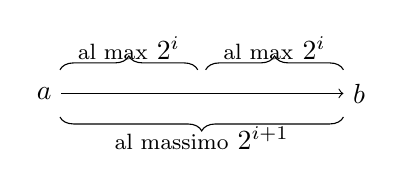
\begin{tikzpicture}
        \node (a) at (0,0) {$a$};
        \node (b) at (4,0) {$b$};
        \draw [->] (a) -- (b);
        \draw [decorate,
            decoration = {brace,mirror,amplitude=5pt}] (0.2,-.3) -- (3.8,-.3) node [midway,below=0.1] {{\footnotesize al massimo} $2^{i+1}$};
        \draw [decorate,
            decoration = {brace,amplitude=5pt}] (0.2,.3) -- (1.95,.3) node [midway,above=0.1] {{\footnotesize al max} $2^i$};
        \draw [decorate,
            decoration = {brace,amplitude=5pt}] (2.05,.3) -- (3.8,.3) node [midway,above=0.1] {{\footnotesize al max} $2^i$};
    \end{tikzpicture}
\end{center}
\begin{eqnarray*}
    &\Updownarrow&\\
    &\exists z \quad \text{Path}(a,z,i) ~\land~ \text{Path}(z,b,i)&
\end{eqnarray*}
In $G$, ci possono volere al massimo $|V|$ passi per raggiungere $v$ da $u$. Quindi
$$
    \text{In } G \text{, } u \text{ raggiunge } v
    ~\Leftrightarrow~
    \text{Path}(u,v,\log|V|) \text{ true}
$$
\begin{center}
    \begin{tikzpicture}
        \draw (0,1.5) -- (10,1.5);
        \draw (0,2) -- (10,2);
        \foreach \x in {0.5,1,3.5,4,5,5.5,6.5} {
          \draw (\x,1.5) -- (\x,2);
        }
        \node[above] at (0.75,1.5) {$\rhd$};
        \node[above] at (3.75,1.5) {;};
        \node[above] at (5.25,1.5) {;};
        \draw [decorate, decoration = {brace,amplitude=5pt}] (1,2.1) -- (3.5,2.1) node [midway,above=0.1] {$G$};
        \draw [decorate, decoration = {brace,amplitude=5pt}] (4,2.1) -- (5,2.1) node [midway,above=0.1] {$u$};
        \draw [decorate, decoration = {brace,amplitude=5pt}] (5.5,2.1) -- (6.5,2.1) node [midway,above=0.1] {$v$};
        \draw [decorate, decoration = {brace,amplitude=5pt}] (1,2.7) -- (6.5,2.7) node [midway,above=0.1] {$n$};

        \draw (0,1) -- (10,1);
        \draw (0,.5) -- (10,.5);
        \foreach \x in {0.5,1} {
          \draw (\x,0.5) -- (\x,1);
        }
        \node[above] at (0.75,0.5) {$\rhd$};
        \draw [decorate, decoration = {brace,mirror,amplitude=5pt}] (1,.4) -- (4.95,.4) node [midway,below=0.1] {Path$(\underbrace{u}_{\log n},\underbrace{v}_{\log n},\underbrace{\log|V|}_{\log n})$};
        \draw [decorate, decoration = {brace,mirror,amplitude=5pt}] (5.05,.4) -- (9,.4) node [midway,below=0.1] {Path$(u,1,\log|V|-1)$};
        \node at (9.75,0) {\dots};
        \draw [decorate, decoration = {brace,mirror,amplitude=5pt}] (1,-1) -- (10.5,-1) node [midway,below=0.1] {stack delle chiamate ricorsive dell'algoritmo};
    \end{tikzpicture}
\end{center}
Nel caso peggiore si ha la tripla $(\log n,\log n,\log n)$ ripetuta $\log n$ volte, quindi SPACE$((\log n)^2)$.\hfill $\square$\medskip

È inefficiente in termini di tempo, ma efficiente in spazio.

\paragraph{Esempio} Il grafo $G$ ha 8 nodi, quindi $|V|=8$, $V=\{1,2,\dots,8\}$, $u=1$, $v=8$. Se scriviamo Path$(1,8,3)$, si sta cercando un cammino da $u$ a $v$ lungo al massimo $2^3$.

\begin{corollary}
    $$
        \text{NSPSACE}(f(n))\subseteq\text{SPACE}(f(n)^2)
    $$
\end{corollary}
\paragraph{Dimostrazione} Sia $\mathcal{N}$ macchina che decide $L$ in spazio $f(n)$. Allora 
$$
    |G_\mathcal{N}(x)| = \gamma^{f(|x|)+\log(|x|)}
$$
Per Savitch 
$$
    \text{SPACE}\left(\log(\gamma^{f(|x|)+\log(|x|)})^2\right) =
    \Theta(f(|x|)^2)
$$
\begin{center}
    \begin{tikzpicture}
        \draw (0,1.5) -- (5,1.5);
        \draw (0,2) -- (5,2);
        \foreach \x in {0.5,1,3} {
          \draw (\x,1.5) -- (\x,2);
        }
        \node[above] at (0.75,1.5) {$\rhd$};
        \draw [decorate,
            decoration = {brace,amplitude=5pt}] (1,2.1) -- (3,2.1) node [midway,above=0.1] {$x$};

        \draw (0,1) -- (5,1);
        \draw (0,.5) -- (5,.5);
        \foreach \x in {0.5,1} {
          \draw (\x,0.5) -- (\x,1);
        }
        \node[above] at (0.75,0.5) {$\rhd$};
        \node[above] at (1.75,0.5) {\dots};

        \node at (2.5,0) {\vdots};

        \draw[->] (5.1,1.75) to [out=0,in=0,looseness=1.5] (5.1,.75);
        \node[right] at (5.5,1.25) {$G_\mathcal{N}(x)$};

        \draw [decorate,
            decoration = {brace,mirror,amplitude=5pt}] (-.4,2.1) -- (-.4,-.5) node [midway,left=0.1] {$\mathcal{N}$};
        \draw [decorate,
            decoration = {brace,amplitude=5pt}] (5.7,1) -- (5.7,-.5) node [midway,right=0.2] {Reachability};
    \end{tikzpicture}
\end{center}
Questo significa che Reachability può essere risolto senza memorizzare il grafo $G_\mathcal{N}(x)$ in un working tape. \hfill $\square$

\begin{corollary}
    $$
        \text{NPSPACE} = \text{PSPACE}
    $$
\end{corollary}

\begin{corollary}
    $$
        \text{N}\mathbb{L} = \text{SPACE}\left( (\log n)^2 \right)
    $$
\end{corollary}
Sappiamo che $\mathbb{L}\subseteq\text{N}\mathbb{L}$. Se dimostrassimo che Reachability $\in$ SPACE$(\log n)$, allora $\mathbb{L}=\text{N}\mathbb{L}$.\medskip

Sappiamo che 
$$
    \text{co-}l = \{ \overline{L} ~|~ L\in l \}
$$
Quindi 
$$
    \text{NPSPACE}=\text{PSPACE}
    ~\Rightarrow~
    \text{co-NPSPACE}= \text{PSPACE}
$$
Inoltre
$$
    \text{co-NPSPACE}(f(n)) \subseteq \text{SPACE}(f(n)^2)
$$
Dato $G_\mathcal{N}(x)$, 
\begin{eqnarray*}
    x\in L &\Leftrightarrow& \text{la configurazione iniziale raggiunge yes (Reachability)}\\
    x\in \overline{L} &\Leftrightarrow& \text{la configurazione iniziale non è in grado di raggiunge yes (Unreachability)}
\end{eqnarray*}
Vogliamo studiare la relazione tra co-NPSPACE$(f(n))$ e NPSPACE$(f(n))$. Qual è la complessità spa\-zia\-le nondeterministica di Unreachability? Dato un grafo $G$ e un nodo $u\in V$, contare il numero di nodi raggiungibili da $u$, con un algoritmo non deterministico e in spazio logaritmico.

% LEZIONE 19
\begin{theorem}[Immerman Szelepcsényi]
    Dato $G=(V,E)$ e $x\in V$, il numero di nodi raggiungibili da $x$ è in NSPACE$(\log n)$.
\end{theorem}
Per un problema di decisione, questo significa che nell'albero di computazione di $\mathcal{N}(x)$ è sufficente uno yes nelle foglie per dire $x\in L$.

Per la computazione di $f:\Sigma\to\mathbb{N}$, i rami non corretti devono terminare con no. Quando un ramo termina con un numero ($f(x)$), siamo certi che il risultato è corretto.

\paragraph{Dimostrazione} Indichiamo con $S(i)$ l'insieme di nodi raggiungibili da $x$ in al massimo $i$ passi. Vogliamo calcolare $|S(|V|-1)|$. Iniziamo da
$$
    S(0) = \{u\}
$$
e quindi $|S(0)|=1$. Poi
\begin{lstlisting}[escapeinside={(*}{*)}]
    for (*$k=1$*) to (*$|V|-1$*)
        compute (*$|S(k)|$*) from (*$|S(k-1)|$*)
\end{lstlisting}
Come si può calcolare $|S(k)|$? 
\begin{lstlisting}[escapeinside={(*}{*)}]
    l := 0
    for (*$u=(1,2,...,|V|)$*)
        if (*$u\in S(k)$*) then l := l+1
\end{lstlisting}
Come si può controllare $u\in S(k)$? L'idea è che 
$$
u\in S
\quad\Leftrightarrow\quad
\exists b\in S(k-1) ~\land~ (\underbrace{u=v ~\lor~ (v,u)\in E}_{G(v,u)})
$$
Quindi
\begin{center}
    \begin{tikzpicture}
        \node (x) at (0,0) {$x$};
        \node (v) at (3,0) {$v$};
        \node (u) at (4,0) {$u$};
        \draw[->, snake it] (x)--(v);
        \draw[->] (v)--(u);

        \draw [decorate,
            decoration = {brace,mirror,amplitude=5pt}] (.2,-.3) -- (2.8,-.3) node [midway,below=0.1] {$\leq x-1$};
        \draw [decorate,
            decoration = {brace,mirror,amplitude=5pt}] (.2,-1.1) -- (3.8,-1.1) node [midway,below=0.1] {$\leq x$};    
    \end{tikzpicture}  
\end{center}
Conosciamo $|S(k-1)|$, possiamo controllare se $u\in S(k)$
\begin{lstlisting}[escapeinside={(*}{*)}]
    m := 0
    reply := false  % diventa true se (*$u\in S(k)$*)
    for (*$v=(1,2,...,|V|)$*)
        if (*$v\in S(k-1)$*)
            m := m+1
            if (*$G(v,u)$*) then reply := true
    if (m = (*$|S(k-1|)$*)) then reply 
    else "no"
\end{lstlisting}
Il passaggio $v\in S(k-1)$ viene eseguito nondeterministicamente.
\begin{lstlisting}[escapeinside={(*}{*)}]
    (*$w_0$*) := (*$x$*)
    for ((*$p = (1,2,...,k-1)$*))
        guess (*$w_p$*)
        check (*$G(w_{p-1},w_p)$*)
    if ((*$w_{k-1}=v$*)) then true 
    else false
\end{lstlisting}
Durante la computazione bisogna memorizzare tutte le variabili $|S(k-1)|$, $k$, l, m, reply, $u$, $v$, $w_p$, $w_{p-1}$, $p$. Queste variabili sono tutte $\in[0,|V|]$. Ognuna di loro richiede spazio $O(\log|V|)$. Poiché non viene mai memorizzato un intero cammino, lo spazio richiesto è proprio $O(\log|V|)$. \hfill$\square$

\begin{corollary}
    $$
        \text{co-NSPACE}(f(n)) = \text{NSPACE}(f(n))
    $$
    con $f(n)\geq\log n$, $f$ propria.
\end{corollary}
\paragraph{Dimostrazione} Utilizzando il Reachability method. $\mathcal{N}$ decide $L$. Dato $G_\mathcal{N}(x)$, $x\in\overline{L}$ sse yes non è raggiungibile (dalla configurazione iniziale, ovvero tutti i nodi finiscono in no). \hfill$\square$




\chapter{Riduzione e Completezza}
Capitolo 8 del libro. Alcuni problemi catturano la difficoltà di un'intera classe di complessità. La logica gioca un ruolo centrale in questo fenomeno.


\section{Riduzioni}
Si vuole risolvere un problema $A$ ``simile'' al problema $B$, e si possiede un algoritmo efficiente per $B$. Si possono eseguire una serie di trasformazioni:
$$
    \underset{\text{input per }A}{x} \to \underset{\text{input per }B}{x'} \to \text{algoritmo} \to \underset{\text{output per }B}{y'} \to \underset{\text{output per }A}{y}
$$
Se una trasformazione ha una complessità molto minore del problema, la complessità rimane la stessa. In particolare, la trasformazione più interessante è quella da $x$ a $x'$, e prende il nome di \textbf{riduzione}.
\begin{definition}[Riduzione]
    Una riduzione da $L_1$ a $L_2$ è
    $$
        R:\Sigma_1^*\to\Sigma_2^* \text{ ~ tale che ~ } x\in L_1 \Leftrightarrow R(x)\in L_2
    $$
    La complessità principale deriva dall'algoritmo per decidere $L_2$.
\end{definition}
$R$ dev'essere computabile in spazio logaritmico.

\paragraph{Esempio (Riduzione)} Si consideri il Graph 3-Coloring ($L_1$): dato un grafo $G=(V,E)$, decidere se è possibile definire $Col:V\to\{r,b,y\}$ tale che se $(u,v)\in E$ allora $Col(u)\neq Col(v)$.

Si consideri SAT ($L_2$): data una formula booleana, decidere se è soddisfacibile o meno. 
$$
    R:\text{Graph 3-Coloring}\to\text{SAT}
$$
ovvero
$$
    R(G) \text{ è soddisfacibile } \Leftrightarrow~ G \text{ è 3-colorabile}
$$
Abbiamo che 
\begin{eqnarray*}
    R(G) &=& \bigwedge_{u\in V} [(r_u\lor b_u\lor y_u) \land 
    (r_u\to \lnot b_u\land \lnot u_u) \land
    (b_u\to \lnot r_u\land \lnot y_u) \land
    (y_u\to \lnot r_u\land \lnot b_u)] \land\\
    & & \bigwedge_{(u,v)\in E} [(r_u\to \lnot r_v) \land (b_u\to \lnot b_v) \land (y_u\to \lnot y_v)]
\end{eqnarray*}
Se in una macchina di Turing con I/O si ha $G$ sul nastro di input e $R(G)$ sul nastro di output, la riduzione deve utilizzare spazio logaritmico sui working tape.

\begin{definition}[$L_1\leq L_2$]
    $L_1$ può essere ridotto a $L_2$ ($L_1\leq L_2$) se esiste una riduzione $R$ da $L_1$ a $L_2$.
\end{definition}

\begin{property} ($\circ$ è la composizione di funzioni)
    \begin{eqnarray*}
        &R_1 \text{ riduzione da } L_1 \text{ a } L_2&\\
        &R_2 \text{ riduzione da } L_2 \text{ a } L_3&\\
        &\Downarrow&\\
        &R_2\circ R_1 \text{ riduzione da } L_1 \text{ a } L_3&
    \end{eqnarray*}
\end{property}
Questo significa che $L_1\leq L_2$ e $L_2\leq L_3$ implica $L_1\leq L_3$. Inoltre, $L_1\leq L_2$ significa che, in termini di complessità, $L_1$ è al più difficile di $L_2$.

\begin{definition}[Chiusura per Riduzione]
    Sia $\mathcal{C}$ una classe di complessità. $\mathcal{C}$ è chiusa per riduzione se
    $$
        L_1\leq L_2 \text{ e } L_2\in\mathcal{C} ~\Rightarrow~ L_1\in\mathcal{C}
    $$
\end{definition}
Si può dimostrare che, ad esempio, P, NP, EXP, $\mathbb{L}$, N$\mathbb{L}$, PSPACE sono tutte chiuse per riduzione. \emph{Esercizio: trovare un esempio di una classe di complessità non chiusa per riduzione.}


\subsection{Completezza}

\begin{definition}[Completezza di una Classe di Complessità]
    Un linguaggio $L$ è completo per una classe $\mathcal{C}$ se
    \begin{enumerate}
        \item $L\in\mathcal{C}$
        \item $\forall L'\in\mathcal{C}$, $L'\leq L$
    \end{enumerate}    
\end{definition}

\begin{center}
    \begin{tikzpicture}
        \draw (0,0) ellipse (2 and 1);
        \node at (-1.8,0.8) {\(\mathcal{C}\)};
    
        \node (l) at (0,0.3) {$\bullet$};
        \node[above right] at (l) {$L$};

        \node (a) at (-1,-.2) {$\bullet$};
        \node (b) at (1.2,-.5) {$\bullet$};
        \node (c) at (0.2,-.7) {$\bullet$};
        \node[text width=3.8cm,right] (d) at (2.5, -.5) {\footnotesize tutti gli altri linguaggi possono essere ridotti a $L$};
        \draw (a) -- (d);
        \draw (b) -- (d);
        \draw (c) -- (d);
    \end{tikzpicture}
\end{center}

\begin{property}
    Se $\mathcal{C}$ e $\mathcal{C}'$ sono classi di complessità 
    \begin{itemize}
        \item chiuse per riduzione, e
        \item $\mathcal{C}\subseteq\mathcal{C}'$, e 
        \item $L'$ è completo per $\mathcal{C}'$, e
        \item $L'\in\mathcal{C}$
    \end{itemize}
    allora $\mathcal{C}=\mathcal{C}'$.
\end{property}

\begin{center}
    \begin{tikzpicture}
        \draw (0,0) ellipse (3 and 2);
        \node at (-2.5,1.5) {\(\mathcal{C}'\)};
        \draw (-.3,-.5) ellipse (2 and 1);
        \node at (-1.6,.6) {\(\mathcal{C}\)};

        \node (lp) at (1.5,1) {$\bullet$};
        \node[above left] at (lp) {$L'$};
        \node[] (tlp) at (3.5, 1.5) {\footnotesize completo};
        \draw[black!30] (lp) -- (tlp);

        \node (l) at (0,-.5) {$\bullet$};
        \draw[->] (lp) -- (l);

        \node[text width=5cm, right] (tl) at (4, 0) {\footnotesize se possiamo dimostrare che $L'$ cade in $\mathcal{C}$, allora tutti gli altri linguaggi possono essere ridotti a $L'$ ($L\leq L', \forall L$), e quindi $\mathcal{C}= \mathcal{C}'$};
        \draw[black!30] (l) -- (tl);
    \end{tikzpicture}
\end{center}



% LEZIONE 20
\subsection{Problema P-Completo: Circuit value}
Una \textbf{formula booleana} è coposta da variabili booleane $x_1,\dots,x_n$, da costanti $0,1$, e da operatori $\land,\lor,\lnot$. Una \textbf{funzione booleana} è 
$$
    \varphi:\{0,1\}^m\to\{0,1\}
$$

\paragraph{Esempio} m=3
$$
    \begin{rcases*}
        \varphi(\overset{x_1}{0},\overset{x_2}{0},\overset{x_3}{0})=1\\
        \varphi(0,1,0)=1\\
        \dots\\
        \varphi(1,1,1)=0
    \end{rcases*} \text{ dominio } |\{0,1\}^3|=8
$$
Questa funzione booleana ha valore 1 solo in due casi, ed è quindi equivalente alla formula booleana
$$
    (\lnot x_1\land \lnot x_2\land \lnot x_3) \lor (\lnot x_1\land 2\land \lnot x_3)
$$
Formule booleane ed espressioni booleane hanno lo stesso potere espressivo.\medskip

I \textbf{circuiti booleani} (boolean circuits) sono equivalenti a formule booleane ed espressioni booleane. Un circuito è composto da \emph{gates}, ovvero nodi di un grafo. I gates sono di tre tipi: variabili, costanti e operazioni.

\begin{center}
    \begin{tikzpicture}
        \node[circle, draw] (x1) at (0,0) {$x_1$};
        \node[circle, draw] (x2) at (2,0) {$x_2$};
        \node[circle, draw] (xm) at (4,0) {$x_m$};
        \node[circle, draw] (and1) at (1,-1) {$\land$};
        \node[circle, draw] (and2) at (3,-1) {$\land$};
        \node[circle, draw] (or) at (2,-2) {$\lor$};

        \draw[->] (x1) -- (and1);
        \draw[->] (x2) -- (and1);
        \draw[->] (x2) -- (and2);
        \draw[->] (xm) -- (and2);
        \draw[->] (and1) -- (or);
        \draw[->] (and1) -- (1,-1.8);
        \draw[->] (and1) -- (0.2,-1.7);
        \draw[->] (and2) -- (or);
        \draw[->] (or) -- (2,-2.8);
    \end{tikzpicture}
\end{center}




\textcolor{Red}{TODO: finire lezione 20}

